\documentclass{mcmthesis}
\mcmsetup{CTeX = false,  
          tcn = {2515324}, problem = \textcolor{red}{E},
          sheet = true, titleinsheet = true, keywordsinsheet = true,
          titlepage = false, abstract = false}
        
\usepackage{newtxtext}     
\usepackage[backend=biber, style=numeric, sorting=none]{biblatex}
\addbibresource{reference.bib}
\usepackage{tocloft}
\usepackage{comment}
\usepackage{float}
\usepackage{colortbl}
\usepackage{xcolor}
\usepackage{graphicx}
\usepackage{subcaption}
\setlength{\cftbeforesecskip}{6pt}
\renewcommand{\contentsname}{\hspace*{\fill}\Large\bfseries Contents \hspace*{\fill}}
\title{From Forest to Farm: Modeling Nitrogen Dynamics
for Sustainable Agriculture}

\date{\today}

\begin{document}

\begin{abstract}
The conversion of forests to farmland significantly alters ecosystem structure and function, often resulting in biodiversity loss and environmental degradation.  This transition is particularly complex due to the interaction of natural ecological processes and human agricultural practices.  This study investigates the ecological consequences of converting forests into farmland, focusing on \textbf{nitrogen cycling} as a key indicator of ecosystem health.  A dynamic modeling approach is employed, utilizing modified Lotka-Volterra equations to simulate nitrogen flow through forest and agricultural food webs.
\par Firstly, we establish a basic model of a \textbf{forest ecosystem's nitrogen cycle (FENCM)}.  This model utilizes a modified Lotka-Volterra approach to simulate the flow of nitrogen through the food web, encompassing producers, consumers at various trophic levels, and decomposers.  The model incorporates key interactions and processes, such as predation, competition, and decomposition, enabling a quantitative assessment of nitrogen dynamics within the forest ecosystem under natural conditions \textbf{(Fig.\ref{fig:model1_result})}. 
The model's parameters are calibrated using data from representative forest ecosystems.

Secondly, we extend the FENCM to establish an \textbf{Agricultural Ecosystem Nitrogen Cycle Model (AENCM)}. This involves incorporating \textbf{human interventions (Sec.\ref{sec:5.4})}, such as planting, harvesting, pesticide and herbicide application, and fertilization.  The AENCM explicitly differentiates between cultivated crops and competing weeds, modeling their interactions and competition for resources. The model also accounts for seasonal variations in growth rates, mortality rates, and human management practices.  This model enables a direct comparison of nitrogen cycling and ecosystem stability under different agricultural strategies, including conventional and organic farming approaches.

Thirdly, to more accurately reflect the complexity of established agricultural ecosystems, the AENCM is further extended into an \textbf{Agricultural Ecosystem-Food Web-nitrogen Cycle Model (AE-FW-NCM)}. This model incorporates a more complex structure of multiple trophic levels and species interactions, reflecting the re-establishment of native species over time as the agricultural ecosystem stabilizes.  The model uses \textbf{predator-prey interaction matrices and competition coefficients }(\textbf{Eq.\ref{eq:model3_food_web}}), along with seasonal and human intervention factors, to precisely simulate nitrogen flux within the ecosystem (\textbf{Fig.\ref{fig:model3_foodWeb_2Chem}}).


Finally, comparative analysis of FENCM, AENCM, and AE-FW-NCM outputs quantifies the impacts of agricultural practices on ecological metrics (species populations, nitrogen fluxes, ecosystem stability).  This highlights trade-offs between yield, biodiversity, and sustainability. Based on our modeling results and comparative analysis, we formulate a set of practical recommendations for farmers considering the adoption of organic farming practices. These recommendations not only emphasize the importance of considering the ecological impacts of agricultural practices but also take into account the practical economic benefits.

\begin{keywords}
Ecosystem Modeling, Agricultural Ecosystems, Nitrogen Cycle, Sustainable Agriculture.
\end{keywords}
\end{abstract}

\maketitle


\tableofcontents       
\thispagestyle{empty}

\newpage

\section{Introduction}

\subsection{Background}
As a pristine forest was felled, towering ancient trees and rich wildlife habitats disappeared, giving way to vast expanses of farmland. The fertile soil became barren, and pests began to infest the crops. In response to this challenge, a human-dominated agricultural ecosystem gradually emerged, establishing a novel food web centered around crops. Nitrogen, as a limiting nutrient, plays a crucial role in determining plant productivity, community structure, and ecosystem function \cite{lebauer2008nitrogen}. The nitrogen cycle in ecosystems serves as a bridge connecting the biotic and abiotic environment. It not only influences the current state of the ecosystem but also drives its long-term succession by regulating interactions among its components—this is what we will explore next.
\begin{figure}[h] 
\centering
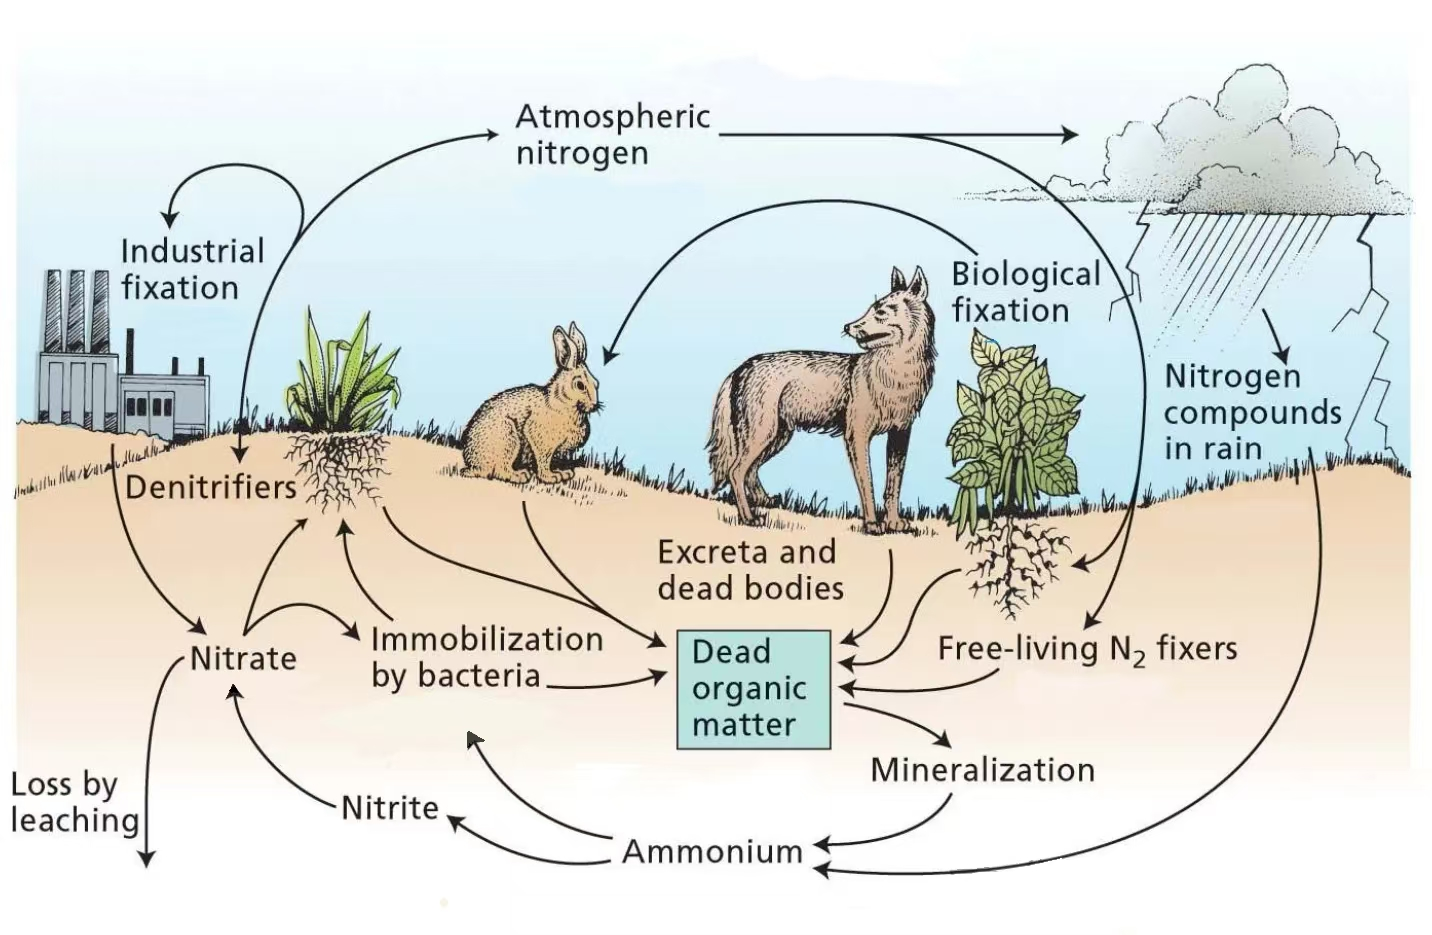
\includegraphics[width=10cm]{figures/background.jpg}
\caption{Schematic Diagram of the Nitrogen Cycle in Ecosystems}
\label{fig:background1}
\end{figure}

\subsection{Restatement of the Problem}
Considering the background information of the conversion of natural ecosystems for agricultural purposes, we aim to address the complex ecological transformations occurring during the conversion of a forest into farmland.  We specifically focus on: 
\begin{itemize}
\item {\bf Task 1:} First, we must develop a foundational mathematical model that accurately represents the original forest ecosystem.
\item {\bf Task 2:} By extending the model, we should establish a food web model for contemporary agricultural ecosystem, aiming to explore the evolution from forest to agricultural ecosystem.
\item {\bf Task 3:} Next, we need to analyze the impacts of agricultural cycles, seasonal variations, pesticides, herbicides, and the reintroduction of native species on agricultural ecosystems.
\item {\bf Task 4:} Furthermore, we should explore the impact of human decisions on agricultural ecosystem by considering alternatives to chemical reliance, such as the adoption of green farming practices and other sustainable pest control methods.
\item {\bf Task 5:}  Finally, we need to offer guidance to farmers, assisting them in identifying effective strategies for implementing organic agricultural practices.
\end{itemize}


\subsection{Our Work}

\begin{figure}[h] 
\centering
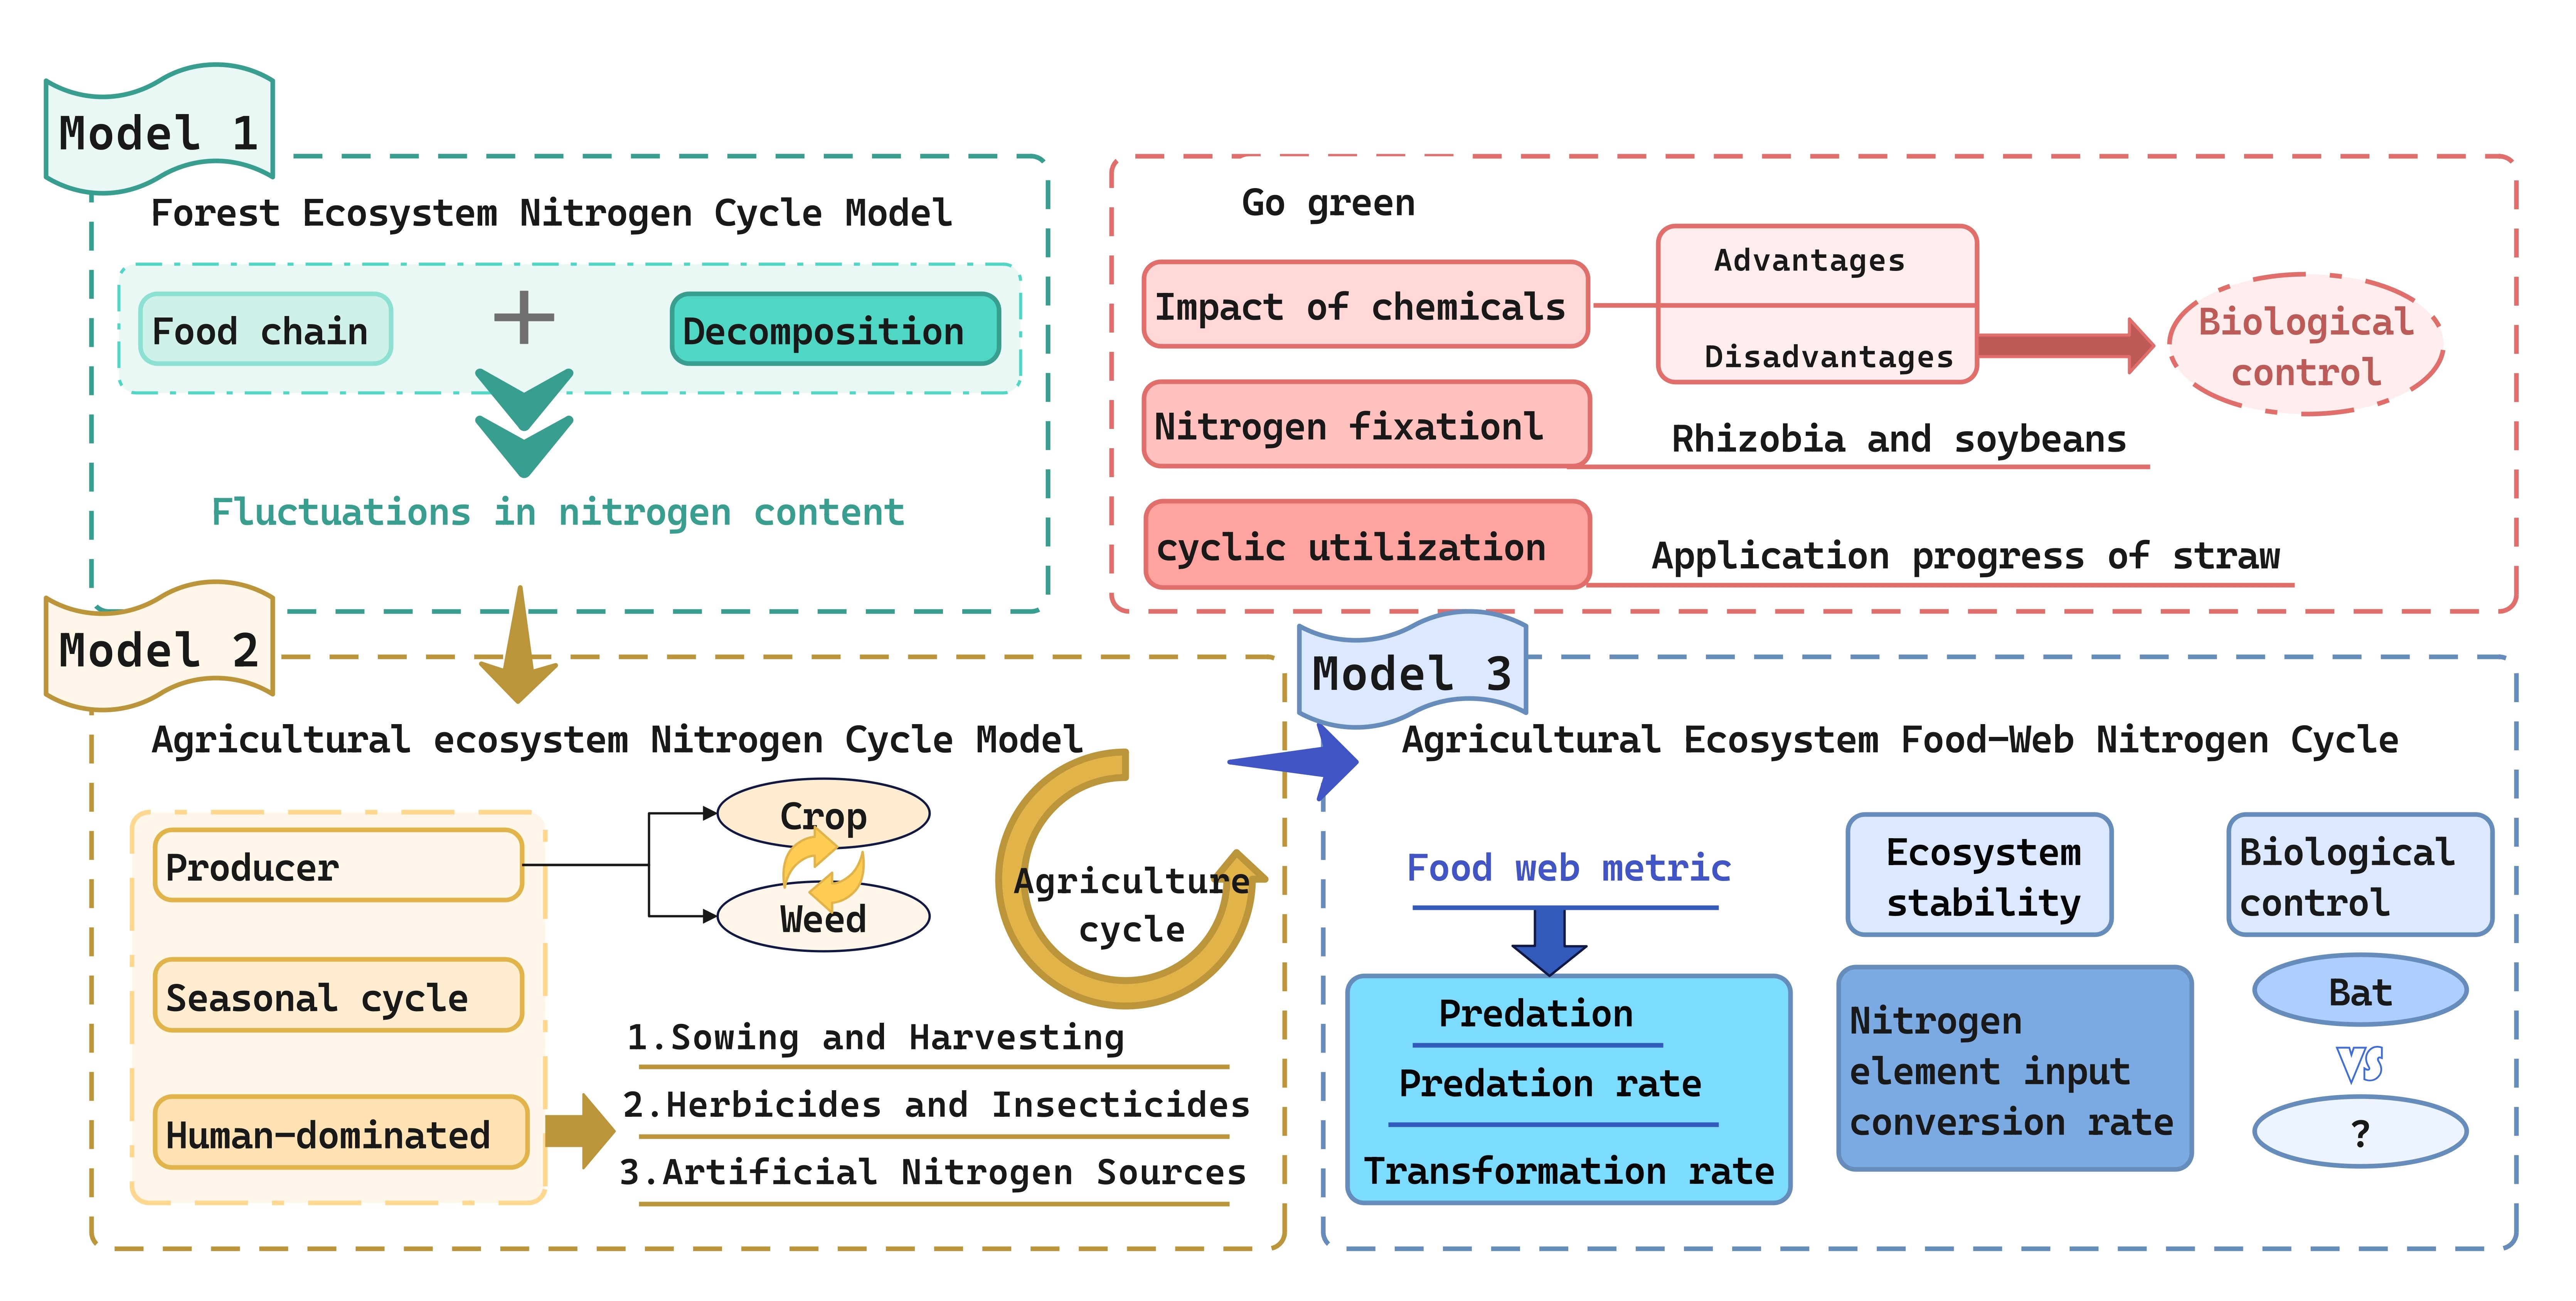
\includegraphics[width=15cm]{figures/our work.jpg}
\caption{Our Work}

\end{figure}
\section{Assumptions and Justification}

To simplify the problem and make it convenient for us to simulate real-life conditions, we make the following basic assumptions, each of which is properly justified.
\begin{itemize}

\item {\bf Assumption 1}: The nitrogen content can serve as a direct indicator of the population of various species in a community.           \\
\textbf{Justification}: Nitrogen is an essential element for plant growth and reproduction, determining both the growth rate and biomass of plants. With rich nitrogen, plant growth accelerates, which in turn can lead to an increase in animal population. Moreover, nitrogen is a critical component of proteins in all living organisms. Therefore, it is reasonable to explore changes in population dynamics through the variation in nitrogen content.

\item {\bf Assumption 2}: In forest and agricultural ecosystems, abiotic environmental factors such as temperature, sunlight and water are abundant and suitable.           \\
\textbf{Justification}: Abiotic environmental resources, such as water and sunlight are crucial for the growth, reproduction, and metabolism of organisms. The long-term stability of ecosystem depends on these factors. Consequently, we assume that in forest and agricultural ecosystem models abiotic resources are abundant and suitable, making research more precise and effective.

\item {\bf Assumption 3}: The total nitrogen content in the ecosystem is conserved.            \\
\textbf{Justification}: We assume that the total nitrogen content in a typical forest ecosystem remains conserved, neglecting nitrogen losses due to exchanges between soil nitrogen salts and atmosphere. However, in the subsequent model (Model II), to accurately reflect the impact of human activities on agricultural ecosystem, we will consider factors such as fertilization and crop harvesting. They will result in significant changes in the nitrogen content in the ecosystem.
\end{itemize}

\section{Notations}


\begin{table}[h]
\centering
\caption{Symbols, Descriptions, and Units}
\begin{tabular}{lll}
\toprule
\textbf{Symbol} & \textbf{Description} & \textbf{Unit} \\
\midrule
$N_{org}$ & Organic Nitrogen & \text{mol/unit area} \\
$N_{inorg}$ & Inorganic Nitrogen & \text{mol/unit area} \\
$N_x$ & Nitrogen content of species $x$ (proportional to population size) & \text{mol/unit area} \\
$\alpha_{x,y}$ & Non-normal mortality rate of species $x$ due to predation by species $y$ & - \\
$\beta_{x,y}$ & Nitrogen utilization rate by species $y$ after preying on species $x$ & - \\
$\gamma_{x}$ & Natural mortality rate of species $x$ & - \\
$c_{x,y}$ & Mortality rate of species $y$ due to competition with species $x$ & - \\
$r$ & Utilization rate of inorganic nitrogen by producers & - \\
$d$ & Total conversion rate of organic nitrogen by decomposers & - \\
$\delta$ & Nitrogen utilization rate by decomposers from organic nitrogen & - \\
\bottomrule
\end{tabular}
\end{table}
\noindent The specific value of those parameters will be given later.

\section{Model 1: Forest Ecosystem Nitrogen Cycle Model}
In the process of forest-to-agriculture conversion, our focus is the establishment of forest ecosystem model. According to Assumption 1, given the important role of nitrogen in the ecosystem cycle, we postulate that nitrogen content directly reflects population density. Therefore, we substitute variations in nitrogen content at different trophic levels to represent changes in population numbers. 

In forest ecosystems, nitrogen transformation occurs in two stages: the first involves nitrogen transfer through the food chain, while the second pertains to the transformation of nitrogen from organic compounds to inorganic compounds under the action of decomposers.The specific process is illustrated in the Figure(\ref{fig:forest_system}).

\begin{figure}[h] 
\centering
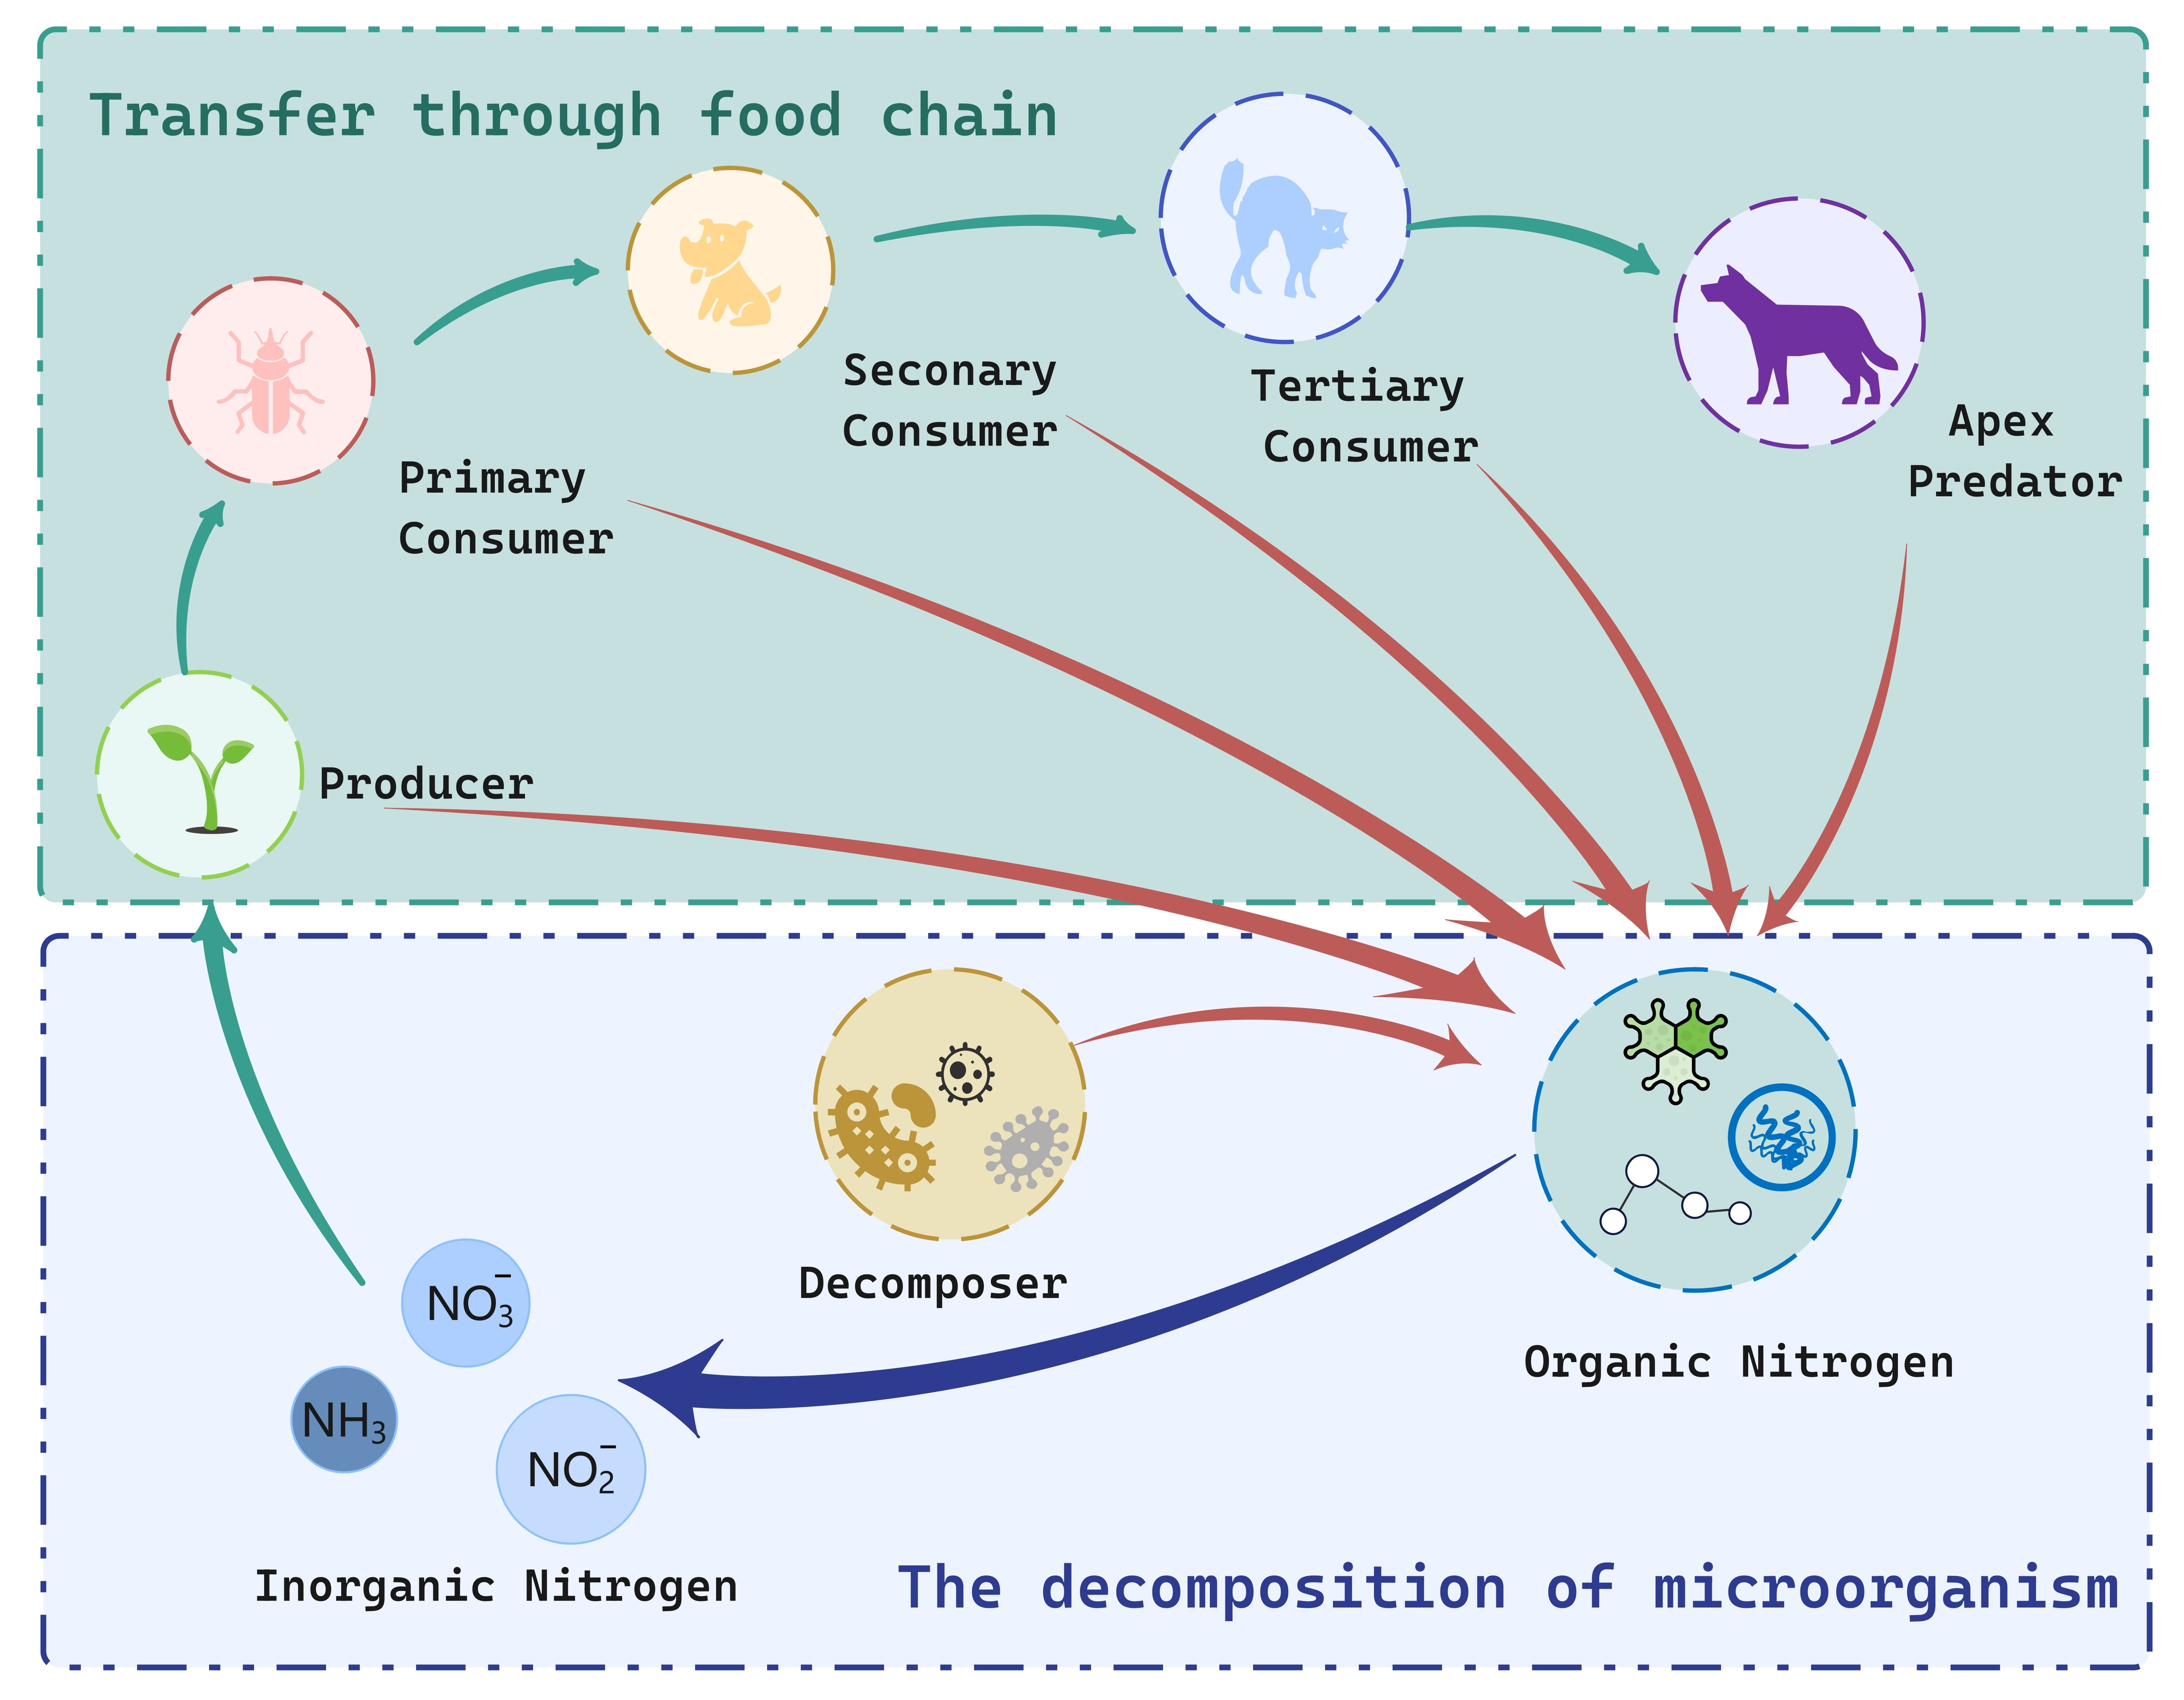
\includegraphics[width=12cm]{figures/forest ecosystem.jpg}
\caption{Forest Ecosystem Nitrogen Cycle Model}
\label{fig:forest_system}
\end{figure}

\subsection{The Nitrogen Flow through the Food Chain}
In forest ecosystems,producers primarily synthesize organic matter via photosynthesis, utilizing inorganic salts and water from the soil. Consumers at different trophic levels acquire nitrogenous compounds through their diet. Thus, nitrogen is predominantly absorbed by plants in inorganic form and transmitted in organic form through the food chain. To model nitrogen flow through the food chain, we first introduce the Lotka-Volterra model\cite{volterra1928variations}, which describes changes in predator $V$ and prey $U$ populations with the following equation.
\begin{align}
   \begin{cases}
        \displaystyle \vspace{10pt}
    \frac{\mathrm{d}U}{\mathrm{d}t} =  r U - \alpha UV \\
        \displaystyle
    \frac{\mathrm{d}V}{\mathrm{d}t} = \beta UV - \gamma V
    \end{cases}
\label{eq: LV}
\end{align}
where:
\begin{itemize} 
\item $r$ represents the reproductive rate of the prey in an environment with abundant resources; 
\item $\alpha$ represents the predation rate of the prey, while $\beta$ indicates the conversion efficiency of the predator post-capture; 
\item $\gamma$ represents the natural mortality rate of the predator. \end{itemize}

In the Lotka-Volterra equation, the constant growth rate $r$, assumes that producers reproduce under conditions of abundant resources. However, according to Assumption 2, it is evident that in the problem we aim to address, the impact of nitrogen on population dynamics must be taken into account. Therefore, we express the reproductive rate of producers as $rN_{inorg}$, where the rate is proportional to the available inorganic nitrogen in the soil. Additionally, we extend equation(\ref{eq: LV}) to accommodate multiple populations within the food chain, resulting in the following equation:
\begin{align}
    \begin{cases}
	\displaystyle \vspace{10pt}
    \frac{\mathrm{d}N_0(t)}{\mathrm{d}t}=rN_{inorg}(t)N_0(t)-\gamma _0N_0(t)-\alpha _{0,1}N_0(t)N_1(t)\\
	\displaystyle \vspace{10pt}
    \frac{\mathrm{d}N_1(t)}{\mathrm{d}t}=\beta _{0,1}N_0(t)N_1(t)-\gamma _1N_1(t)-\alpha _{1,2}N_1(t)N_2(t)\\
    \quad\quad\quad\quad\quad\quad\quad\quad\quad \quad\quad\quad\quad\vdots\\
	\displaystyle \vspace{10pt}
    \frac{\mathrm{d}N_{k-1}(t)}{\mathrm{d}t}=\beta _{k-2,k-1}N_{k-2}(t)N_{k-1}(t)-\gamma _{k-1}N_{k-1}(t)-\alpha _{k-1,k}N_{k-1}(t)N_k(t)\\
	\displaystyle
    \frac{\mathrm{d}N_k(t)}{\mathrm{d}t(t)}=\beta _{k-1,k}N_{k-1}(t)N_k(t)-\gamma _kN_k(t)\\
\end{cases}
\label{eq:forest_food_chain}
\end{align}
where
\begin{itemize} 
\item $N_0(t)$ represents the nitrogen content of the producers, $N_k(t)$ $(k \geq 1)$ denotes the nitrogen content of the $k$-th consumer at time $t$, and $N_{inorg}(t)$ refers to the inorganic nitrogen content in the environment at time $t$;
\item $r$ represents the reproduction rate of the producers. According to Assumption 2, under conditions where other environmental resources are abundant and suitable, the growth rate primarily depends on the inorganic nitrogen salts present in the environment; 
\item $\gamma$ represents the natural mortality rate of the species; 
\item $\alpha_{i,j}$ represents the non-natural mortality rate of species $i$ caused by predation by species $j$, and $\beta_{i,j}$ refers to the nitrogen conversion rate for growth and reproduction after species $j$ preys on species $i$. 
\end{itemize}

\subsection{The Nitrogen Flow through Decomposers and the Food Chain}
The feces and carcasses of producers and consumers in the food chain are transformed by decomposers from nitrogenous organic compounds into nitrogenous inorganic compounds. Then they can be directly utilized by primary producers. The specific process is illustrated in Figure(\ref{fig:decomposer_nitrogen}).
\begin{figure}[h] 
\centering
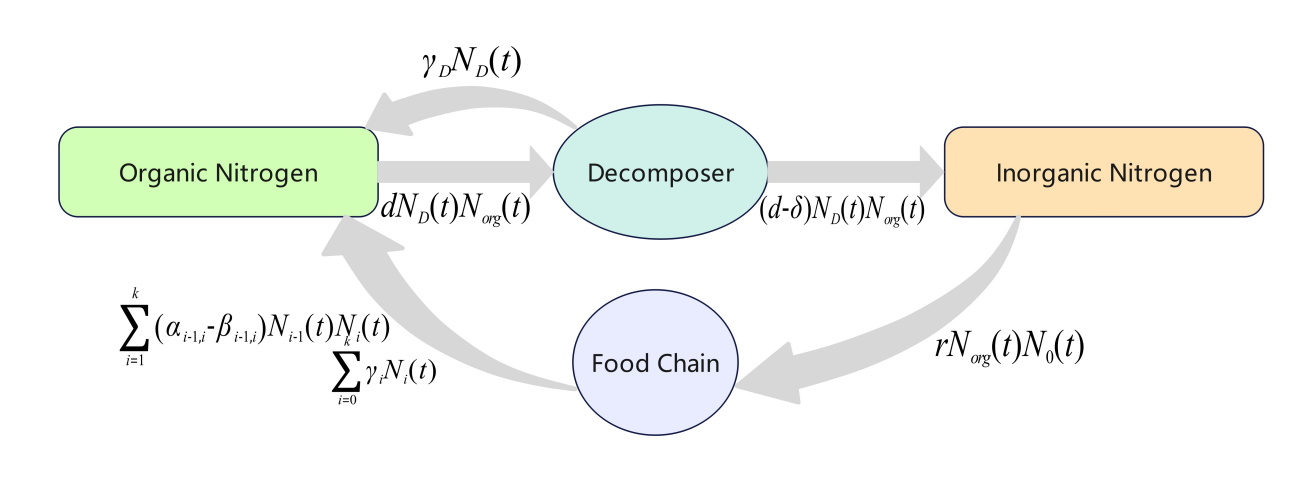
\includegraphics[width=12cm]{figures/decomposer&nitrogen.png}
\caption{Nitrogen Cycle through Decomposer and Food Chain}
\label{fig:decomposer_nitrogen}
\end{figure}

Feces and carcasses of various trophic levels and decomposers  will be transformed into nitrogenous organic compounds. Simultaneously, consumers at different trophic levels absorb a portion of nitrogenous organic compounds from their prey for growth and reproduction.Based on this, we establish equation(\ref{eq:model1_organic_nitrogen}) to describe the changes in organic nitrogen content in the environment.
\begin{align}
    \displaystyle 
    \label{eq:model1_organic_nitrogen}
    \frac{\mathrm{d}N_{org}(t)}{\mathrm{d}t} = \sum_{i=1}^k{\left( \alpha _{i-1,i}-\beta _{i-1,i} \right) N_{i-1}(t)N_i(t)} + \sum_{i=0}^k{\gamma _iN_i(t)} + \gamma _D N_D(t) - d N_D(t) N_{org}(t) 
\end{align}
where
\begin{itemize} 
\item $N_{org}$ represents the organic nitrogen content in the environment, while $N_D$ denotes the nitrogen content within decomposers; 
\item $\gamma_D$ represents the mortality rate of decomposers, and $d$ refers to the conversion rate of organic matter by decomposers in the environment. 
\end{itemize}
We formulate equation(\ref{eq:model1_decomposer}) to represent the variation of nitrogen among decomposers. In this model, $\delta$ denotes the growth and reproduction rate of decomposers. The primary source of nitrogen within decomposers is the organic nitrogen from the remains of producers and consumers, and its main destination is natural mortality.
\begin{align}
      \displaystyle 
    \frac{\mathrm{d}N_D(t)}{\mathrm{d}t} = \delta N_D(t) N_{org}(t) - \gamma _D N_D(t)
    \label{eq:model1_decomposer}
\end{align}
where $\delta$ represents the utilization rate of inorganic nitrogen by decomposers, which is used for their growth and reproduction.

For inorganic nitrogen variation, we primarily investigate the fraction that is available to producers, specifically the inorganic nitrogen present in the soil. We have developed equation (\ref{eq:model1_inorganic_nitrogen}) to represent the changes in nitrogen content within the inorganic environment. The main source of this nitrogen is the conversion of organic nitrogen by decomposers. A portion is used for their own growth and reproduction, while the remainder is primarily directed toward uptake by producers.
\begin{align}
    \displaystyle 
    \frac{\mathrm{d}N_{inorg}(t)}{\mathrm{d}t} = \left( d - \delta \right) N_D(t) N_{org}(t) - r N_{org}(t) N_0(t) 
    \label{eq:model1_inorganic_nitrogen}
\end{align}
where $N_{inorg}$ represents the inorganic nitrogen content in the environment.

\subsection{Model Solving}
Using data from representative global forests as a reference, we assigned appropriate values to the parameters in the FENCM model. Then we adjusted them to examine the model's performance under varying parameters and initial conditions. Ultimately, we determined the model parameters to be those presented in table (\ref{tab:model1_initial_values}).
\begin{table}[H]
\centering
\caption{System Initial Values and Parameters}
\scriptsize
\label{tab:model1_initial_values}
\begin{tabular}{lll|lll}
\hline
\textbf{Initial Value} & \textbf{Variable} & \textbf{Value} & \textbf{Parameter} & \textbf{Symbol} & \textbf{Value} \\
\hline
Primary Producers & $N_0(0)$ & 10 & Producer Growth Rate & $r$ & 0.1 \\
Primary Consumers & $N_1(0)$ & 3 & Death Rates & $\gamma_0,\gamma_1,\gamma_2,\gamma_3$ & 0.01, 0.2, 0.05, 0.3 \\
Secondary Consumers & $N_2(0)$ & 2 & Predation Rates & $\alpha_{0,1},\alpha_{1,2},\alpha_{2,3}$ & 0.02, 0.05, 0.03 \\
Tertiary Consumers & $N_3(0)$ & 1 & Conversion Efficiencies & $\beta_{0,1},\beta_{1,2},\beta_{2,3}$ & 0.015, 0.04, 0.015 \\
Organic Nitrogen & $N_{org}(0)$ & 5 & Decomposition Rate & $d$ & 0.2 \\
Decomposers & $N_D(0)$ & 100 & Decomposer Absorption & $\delta$ & 0.12 \\
Inorganic Nitrogen & $N_{inorg}(0)$ & 50 & Decomposer Death Rate & $\gamma_D$ & 0.5 \\
\hline
\end{tabular}
\end{table}

Under the given parameters, we solve the model, and the results are presented in Figure(\ref{fig:model1_result}).
\begin{figure}[h] 
\centering
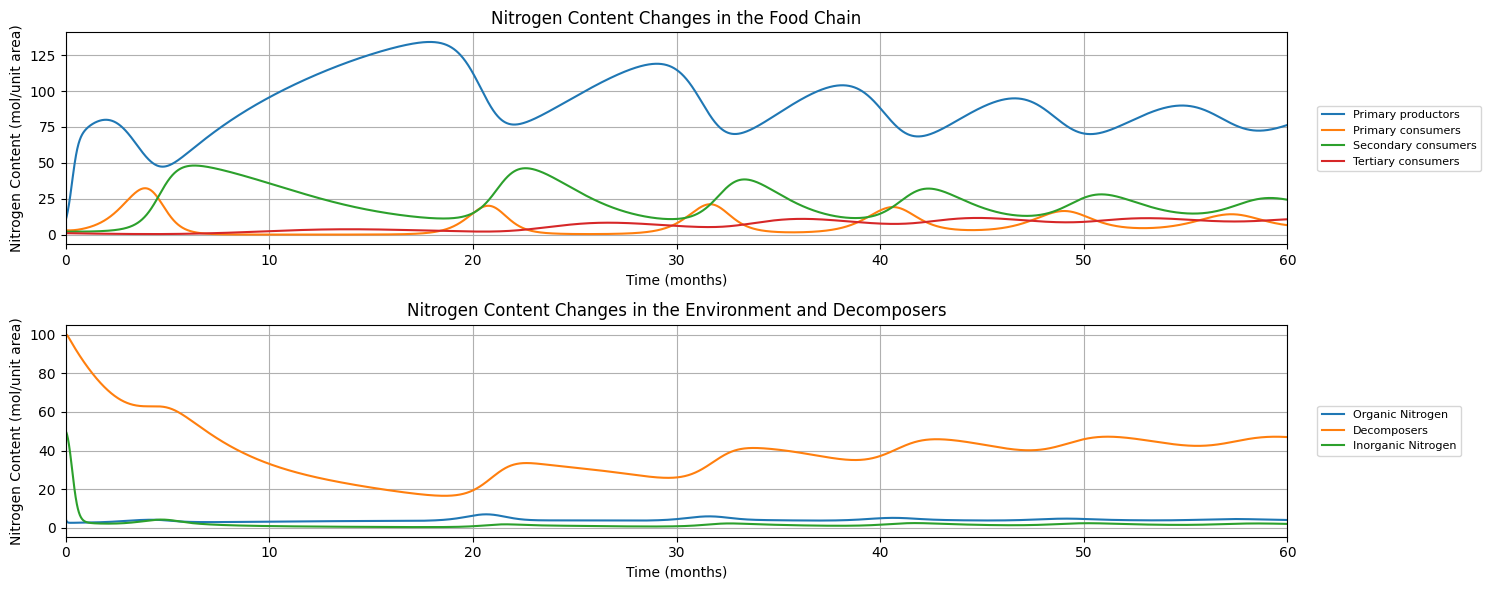
\includegraphics[width=\textwidth]{figures/model1_result.png}
\setlength{\abovecaptionskip}{-0.5cm} % 调整图片标题与图片之间的距离
\caption{The result of FENCM}
\label{fig:model1_result}
\end{figure}

From the figure, we can observe that after 20 months($t$=20), the nitrogen content of producers and various trophic levels of consumers in the food chain begins to exhibit a regular cyclical pattern. Concurrently, the concentrations of organic and inorganic nitrogen in the environment gradually stabilize. Additionally, it is evident from our simulation results that inorganic nitrogen levels in the environment stabilize at relatively low levels, with a greater proportion of nitrogen being retained within the biota. This observation is consistent with findings from previous studies \cite{GEISSELER2010}.

It is noteworthy that in the figure, the cyclical variations in nitrogen content across different trophic levels exhibit a trend of “reciprocal increase and decrease”. According to ecological principles, adjacent trophic levels are characterized by predator-prey relationships. When the population of prey increases, it provides more food for predators, leading to an increase in their population. As predator numbers rise, the prey population declines, resulting in a reduction in the food supply for predators, which in turn causes a decrease in their population. As a result, the interaction between predators and prey establishes a negative feedback mechanism. It includes periodic fluctuations in their population sizes, typically following a pattern of “early increase, early decrease; later increase, later decrease”, or “reciprocal increase and decrease”. Our fitting results effectively demonstrate this characteristic, highlighting the success of the FENCM model.

\section{Model 2: Agriculatural Ecosystem Nitrogen Cycle Model}
Compared to forest ecosystems, the most significant characteristic of agricultural ecosystems is their human-driven nature. Consequently, we incorporate factors related to human activities into the forest nitrogen cycle model to construct an agricultural ecosystem nitrogen cycle model (AENCM).
\subsection{Producer Classification: Crop Competition with Weeds}
\label{sec:5_1}
Within agricultural ecosystems, producers are primarily divided into two categories: one consists of crops cultivated by humans, which typically hold a dominant position in terms of numbers, and the other comprises naturally occurring weeds. Given that agricultural ecosystems are predominantly controlled by human actions, the growth conditions of both are influenced by human activities. The sowing and harvesting processes of crops lead to regular fluctuations in their numbers in accordance with agricultural cycles, while regular weeding practices by humans somewhat suppress weed populations. Based on the competitive interactions between these two producers, we establish equations for the nitrogen content dynamics of crops and weeds:
\begin{align}
\label{eq:model2_competition}
    \begin{cases}
	\displaystyle \vspace{10pt}
    \frac{\mathrm{d}N_{w}(t)}{\mathrm{d}t}=r_{w}N_{inorg}(t)N_{w}(t)-\gamma _{w}N_{w}(t)-\alpha _{w,1}N_{w}(t)N_1(t)-c_{c,w}N_{c}(t)N_{w}(t)  \\
    % 这里增加了垂直间距
    \displaystyle
	\frac{\mathrm{d}N_{c}(t)}{\mathrm{d}t}=r_{c}N_{inorg}(t)N_{c}(t)-\gamma _{c}N_{c}(t)-\alpha _{c,1}N_{c}(t)N_1(t)-c_{w,c}N_{w}(t)N_{c}(t)
\end{cases}
\end{align}
where
\begin{itemize}
    \item $N_w(t)$ represents the nitrogen content in weeds at time $t$, and $N_c(t)$ represents the nitrogen content in crops at time $t$;
    \item $r_w$ and $r_c$ represent the reproduction rates of weeds and crops;
    \item $\gamma_w$ and $\gamma_c$ represent the natural mortality rates of weeds and crops;
    \item $c_{c,w}$ indicates the unnatural mortality of weeds due to competition with crops, and $c_{w,c}$ indicates the unnatural mortality of crops due to competition with weeds.
\end{itemize}
\subsection{Agricultural Ecosystem Nitrogen Cycle Model}
Due to human cultivation, during the transition from forests to farmland, many species opt to migrate because of habitat fragmentation and loss, particularly insectivorous birds, reptiles, and large mammals \cite{Laurance_Vasconcelos_Lovejoy_2000}. Consequently, we posit that within agricultural ecosystems, the higher-level consumers previously present in forest ecosystems have all departed, leaving food chains that encompass only producers, primary consumers, and secondary consumers. Based on the above analysis, we establish the following equations to describe the changes in nitrogen content of primary and secondary consumers:
\begin{align}
\label{eq:model2_food_chain}
    \begin{cases}
        \displaystyle \vspace{10pt}
    \frac{\mathrm{d}N_1(t)}{\mathrm{d}t}=\beta _{w,1}N_{w}(t)N_1(t)+\beta _{c,1}N_{c}(t)N_1(t)-\gamma _1N_1(t)-\alpha _{1,2}N_1(t)N_2(t)\\
        \displaystyle
	\frac{\mathrm{d}N_2(t)}{\mathrm{d}t}=\beta _{1,2}N_{1}(t)N_2(t)-\gamma _2N_2(t)\\
\end{cases}
\end{align}
In which, the nitrogen intake process by primary consumers is bifurcated into two parts, one from weeds and the other from crops. Due to the distinct characteristics of these two types of plants, it is believed that primary consumers exhibit different preferences for each, represented by $\beta _{w,1}$ and $\beta _{c,1}$ in the aforementioned equations.

During the process of decomposition in agricultural ecosystems, organic nitrogen content is derived from three major sources: the natural death of consumers and decomposers, nitrogenous organic matter assimilated by consumers from the preceding trophic level but not utilized for their own growth, and the remains from the competitive exclusion of weeds and crops. Regarding the dynamics of decomposers and inorganic nitrogen content, it is assumed to be analogous to that of  forest ecosystem. In summary, we establish the following equations:
\begin{align}
\label{eq:model2_environment}
\begin{cases}
    \displaystyle \frac{\mathrm{d}N_{org}(t)}{\mathrm{d}t} 
   =  &\left( \alpha _{1,2} - \beta _{1,2} \right) N_1(t) N_2(t) + \gamma_1 N_1(t) + \gamma_2 N_2(t) + \gamma_D N_D(t) \\
   & - d N_D(t) N_{org}(t) 
     + \left( \left( \alpha_{w,1} - \beta_{w,1} \right) N_w(t) + \left( \alpha_{c,1} - \beta_{c,1} \right) N_c(t) \right) N_1(t) \\
    & + \gamma_w N_w(t) + \gamma_c N_c(t) + \left( c_{w,c} + c_{c,w} \right) N_c(t) N_w(t) \\
    \vspace{10pt} 
    \displaystyle \frac{\mathrm{d}N_D(t)}{\mathrm{d}t} 
    =  &\delta N_D(t) N_{org}(t) - \gamma_D N_D(t) \\
    \displaystyle \frac{\mathrm{d}N_{inorg}(t)}{\mathrm{d}t}
    =  &\left( d - \delta \right) N_D(t) N_{org}(t) - r_w N_{inorg}(t) N_w(t) - r_c N_{inorg}(t) N_c(t)
\end{cases}
\end{align}

Although generally similar to equations (\ref{eq:model1_organic_nitrogen}) ,(\ref{eq:model1_decomposer}) and (\ref{eq:model1_inorganic_nitrogen}), we have taken into account the competition between crops and weeds in agricultural ecosystems, as well as the distinct preferences of primary consumers for both, introducing $c_{c,w}$ and $c_{w,c}$, to extend and refine the equations.

Forest ecosystems exhibit a high degree of species complexity and richness, with overall stability being notably high. The diverse community of species and ecological functions enable them to effectively respond to external disturbances brought about by seasonal cycles. In contrast, agricultural ecosystems typically comprise only a few crop species, resulting in lower biodiversity. Production activities are largely contingent upon seasonal climatic conditions, thus the stability and productivity of agricultural ecosystems are often subject to the influence of seasonal fluctuations. Moreover, agricultural ecosystems frequently necessitate human management and intervention, such as sowing, harvesting, weeding, and fertilization. Consequently, to better understand the dynamics, it is imperative to discuss the impact of seasonal cycles and human decision-making on agricultural ecosystems.
\subsection{Seasonal cyclic factor}
Seasonality is one of the pivotal factors in the agricultural production process, encompassing climate variation, crop growth cycles, and soil conditions, among others. In agricultural ecosystems, seasonal fluctuations directly impact the growth, maturation, and mortality of crops and weeds, thereby indirectly influencing the population of primary consumers such as pests.

Accordingly, we posit that seasonal factors primarily affect the reproductive rates, natural mortality rates of both producers, and the natural mortality of primary consumers, establishing the equations as follows:
\begin{align}
\label{eq:model2_season}
\begin{cases}
\displaystyle \vspace{10pt}
r_w\left( t \right) =r_{w}^{0}+r_{w}^{s}\sin \left( \frac{2\pi t}{T}+\phi \right) 
\\
\displaystyle \vspace{10pt}
r_c\left( t \right) =r_{c}^{0}+r_{c}^{s}\sin \left( \frac{2\pi t}{T}+\phi \right) 
\\
\displaystyle \vspace{10pt}
\gamma _{1}\left( t \right) =\gamma _1^{0} +\gamma _{1}^{s}\sin \left( \frac{2\pi t}{T}+\phi + \pi \right)
\\
\displaystyle \vspace{10pt}
\gamma _{w}\left( t \right) =\gamma _w^{0} +\gamma _{w}^{s}\sin \left( \frac{2\pi t}{T}+\phi + \pi \right)
\\
\displaystyle
\gamma _{c}\left( t \right) =\gamma _c^{0} +\gamma _{c}^{s}\sin \left( \frac{2\pi t}{T}+\phi + \pi \right)
\end{cases}
\end{align}
where
\begin{itemize}
    \item $r_{w}^{0}$ and $r_{c}^{0}$ represent the baseline production rates of weeds and crops, while $\gamma_1^{0}$,  $\gamma_w^{0}$ and $\gamma_c^{0}$ represent the baseline natural mortality rates of primary consumers, weeds, and crops;
    \item $r_{w}^{s}$, $r_{c}^{s}$, $\gamma_{1}^{s}$, $\gamma_{w}^{s}$ and $\gamma_{c}^{s}$ exhibit annual periodicity, they are adjustments to the reproduction and natural mortality rates due to seasonal cyclical variations.
\end{itemize}

Incorporating seasonal cyclic factors, by simultaneously solving equations (\ref{eq:model2_competition}), (\ref{eq:model2_food_chain}), (\ref{eq:model2_environment}), and (\ref{eq:model2_season}), numerical simulations of the agricultural ecosystem can be conducted. The simulation results are depicted in Figure \ref{fig:model2_season}. 

\begin{figure}[h] 
\centering
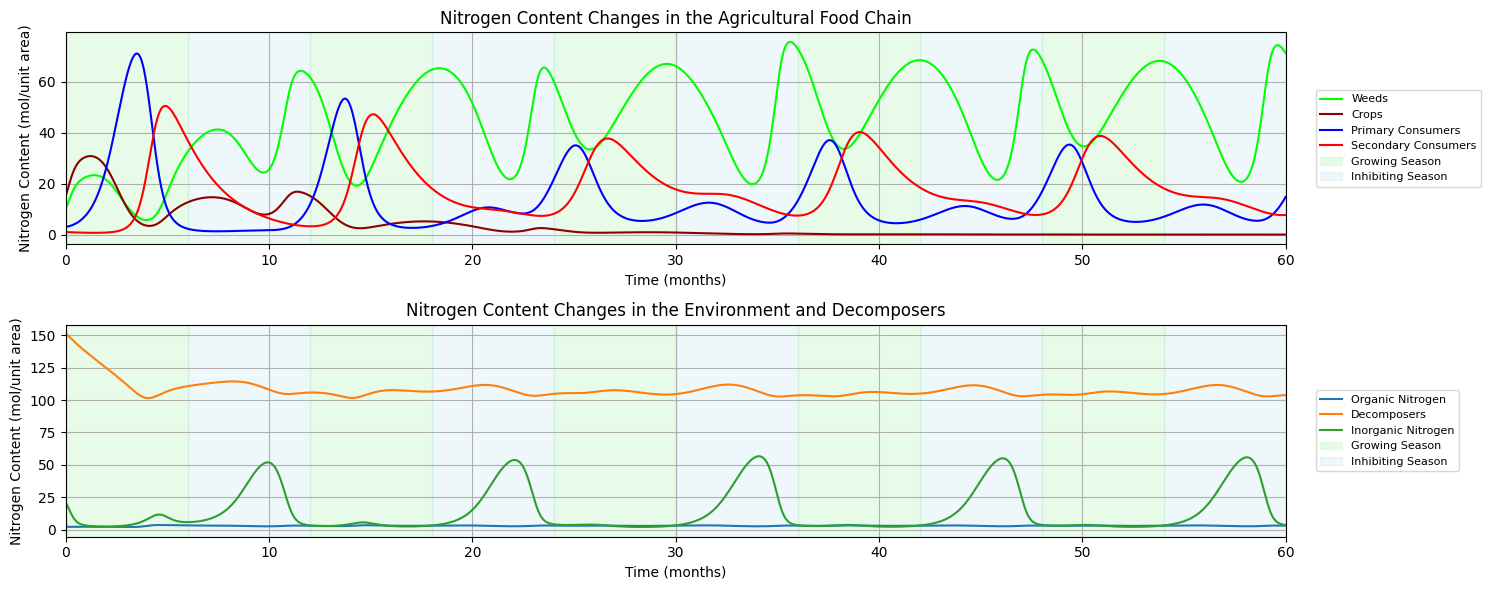
\includegraphics[width=\textwidth]{figures/model2_season.png}
\setlength{\abovecaptionskip}{-0.5cm} % 调整图片标题与图片之间的距离
\caption{Seasonal Cycle Factors Affecting Agricultural Ecosystems}
\label{fig:model2_season}
\end{figure}

As shown in Figure \ref{fig:model2_season}, the growth of weeds exhibits an annual 'two-peak' pattern, occurring because weeds reproduce abundantly during the spring and summer growing seasons, leading to an increase in population size. However, as the number of consumers increases, the weed population subsequently declines, consistent with the 'rise and fall' trend identified in the solutions of the preceding FENCM model. Upon entering the autumn and winter suppression seasons, the reproductive rate of weeds slows, mortality rates rise, and the population size decreases due to seasonal influences such as climate, moisture, and soil conditions.

At the same time, based on the simulation results above, it can be observed that during the first spring and summer growth season, the crop population reaches its first peak after abundant reproduction, then immediately declines, and thereafter remains at a lower level. This may be due to the increase in the number of primary and secondary consumers, enhancing their predation capacity on crops, and during the interspecific competition between crops and weeds, the competitive intensity of weeds is higher, exerting an inhibitory effect on crop growth and reproduction. 

Additionally, we observed that the nitrogen content in crops is almost depleted after 20 months. This may be because the species diversity of weeds in agricultural ecosystems is higher, exerting stronger competitive pressure on crops, and their growth and reproduction rates are faster, thus quickly placing crops at a competitive disadvantage.

However, we must also consider that agricultural ecosystems are artificially created, and the role of human cyclical cultivation in these ecosystems is an indispensable part. Therefore, in the following section, we will continue to discuss the impact of humans in agricultural ecosystems.
\subsection{Impact of Humans on Agricultural Ecosystems}\label{sec:5.4}
The cyclical cultivation by humans is primarily manifested in agricultural cycles. An agricultural cycle refers to the complete process from sowing to harvest, encompassing all stages of crop growth, typically including soil preparation, sowing, seedling, weeding, pest control, fertilization, harvesting, and post-harvest handling, etc., and is accompanied by the transformation of organic and inorganic nitrogen, as shown in Figure \ref{fig:Agriculture_cycle}. The agricultural cycle is not only related to crop growth but also directly affects the state of the agricultural ecosystem, and we will discuss the impact of each stage of the agricultural cycle on the agricultural ecosystem in the following sections.
\begin{figure}[h] 
\centering
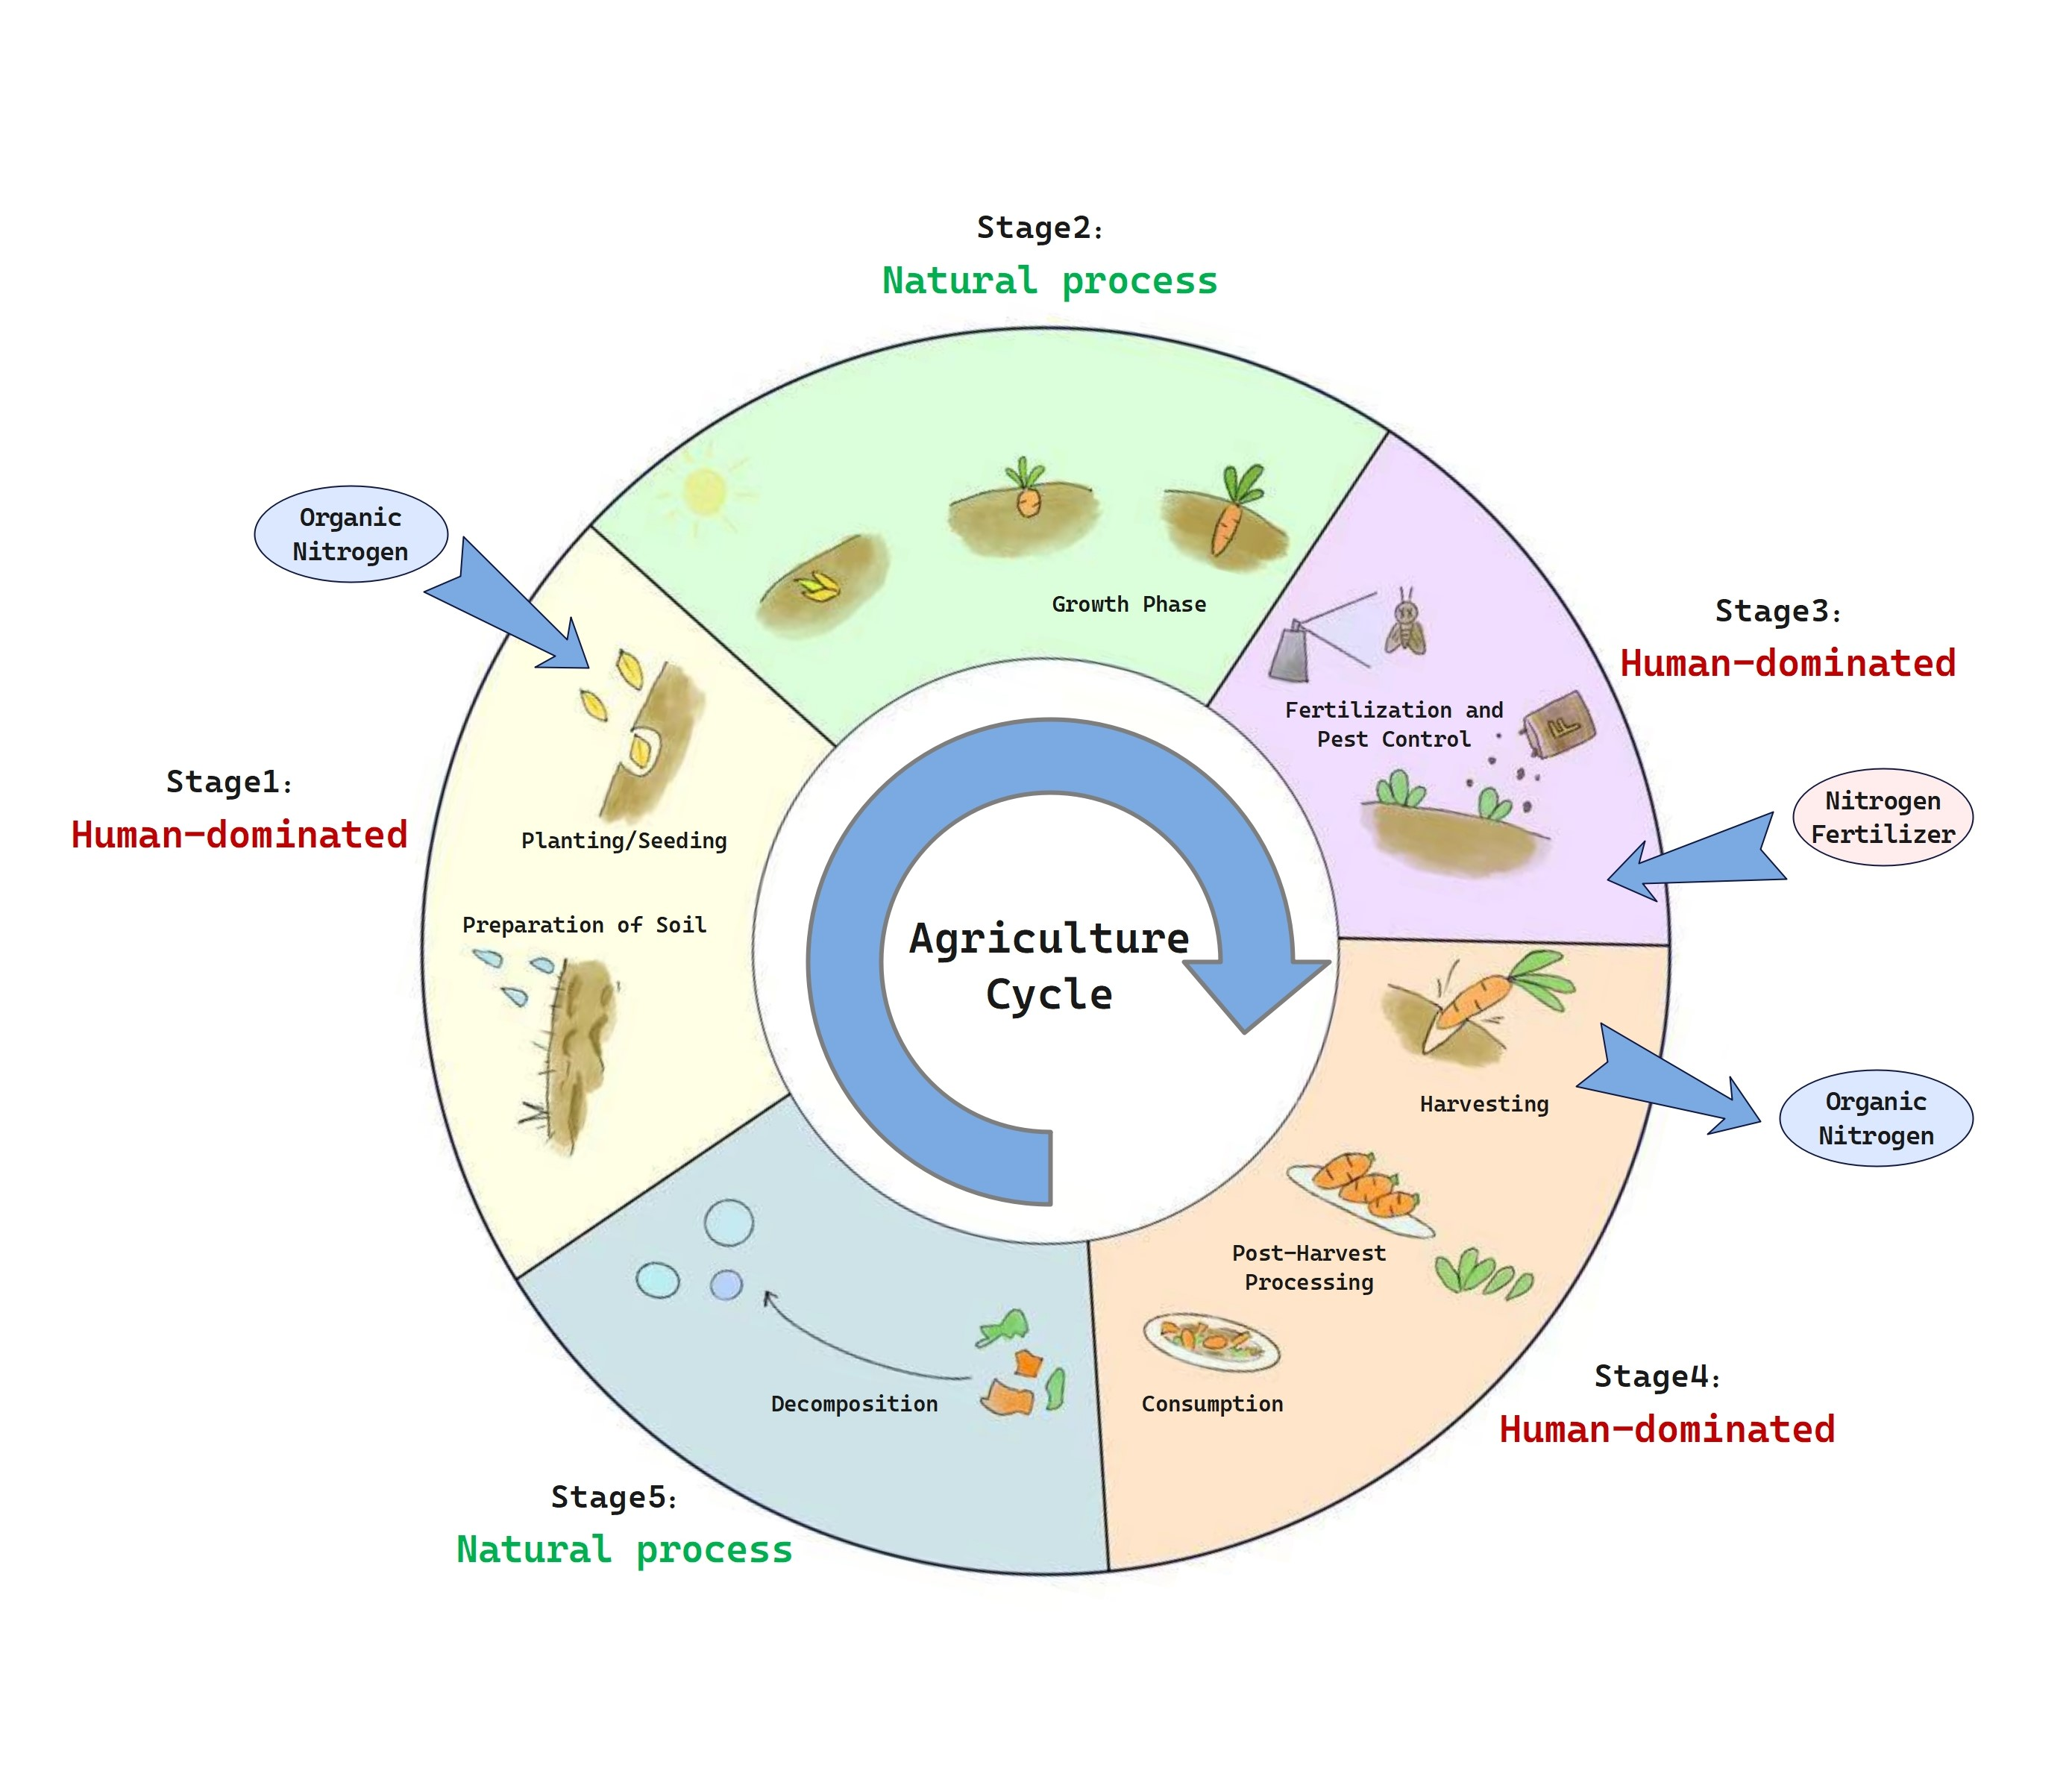
\includegraphics[width=10cm]{figures/Agriculture cycle.jpg}
\caption{Agriculture cycle}
\label{fig:Agriculture_cycle}
\end{figure}
\subsubsection{Sowing and Harvesting}

Human sowing and harvesting are indispensable parts of the agricultural cycle, playing a crucial role in agricultural ecosystems. Initially, sowing can alter the vegetation structure and species composition of the land. By selective planting, it controls the competition between weeds and crops, thereby promoting the growth of crops; harvesting is another important stage in the agricultural cycle. It often involves soil cultivation and resowing, which can affect soil structure, crop growth, and ecosystem productivity. Therefore, based on equation (\ref{eq:model2_competition}), we modify it to obtain the equation for the change in nitrogen content of crops after introducing the factors of sowing and harvesting:
\begin{align}
\label{eq:organic_nitrogen_with harvest}
    \frac{\mathrm{d}N_c}{\mathrm{d}t}=&r_cN_{inorg}N_c-\gamma _cN_c-\alpha _{c,1}N_cN_1-c_{w,c}N_wN_c \nonumber \\  
 &-\boxed{\delta _D\left( t-t_{h}^{0}-T_an_a \right) N_c\left( t \right)}
+ \boxed{S\delta _D\left( t-t_{s}^{0}-T_an_a \right)}
\end{align}
where
\begin{itemize}
    \item $T_a$ represents the duration of an agricultural cycle; $n_a = \lfloor \frac{t}{T_a} \rfloor$ denotes the count of agricultural cycles;
    \item $\delta_D$ signifies the Dirac delta function of a single pulse, defined as $\delta_D(x) = 0 (\forall x \neq 0)$, and $\int_{-\infty}^{+\infty}f(x)\delta_D(x) = f(0)(\forall f(x)\in \mathbb{R})$;
    \item $t_h^0$ and $t_s^0$ represent the times of starting harvesting and sowing;
    \item $S$ indicates the organic nitrogen content at sowing.
\end{itemize}

Considering that only a portion of the harvested crop can be used as human food, the remaining organic nitrogen is stored in the straw. The use of straw is discussed in section \ref{sec:crops_residue}, where we temporarily assume that the straw is harvested and taken out of the ecosystem along with the crops. We can also define a harvest function to represent the organic nitrogen used for human consumption:
\begin{align}
\label{eq:harvest_function}
    H(t) = h \cdot \int_0^t \delta_D( x - t_{h}^{0} - T_{a_n} ) N_c (x) \mathrm{d}x
\end{align}

Here, $h$ is the harvest coefficient, which is related to the type of plant and its developmental status. The harvest function defined above can be used to measure the nitrogen yield of agriculture.

Without considering the effects of chemical substances, we can simultaneously solve equations (\ref{eq:organic_nitrogen_with harvest}) and (\ref{eq:harvest_function}) to perform numerical simulations of the agricultural ecosystem, with the results shown in Figure \ref{fig:model2_no_chem}. From the simulation results, we can see that the total amount of nitrogen in the environment undergoes an abrupt decrease after the first harvest at $(t = 24 \times \text{days})$. This is because during the harvesting process, the nitrogen contained in the crops also leaves the agricultural ecosystem, thus reducing the total nitrogen content in the entire ecosystem.
\begin{figure}[h] 
\centering
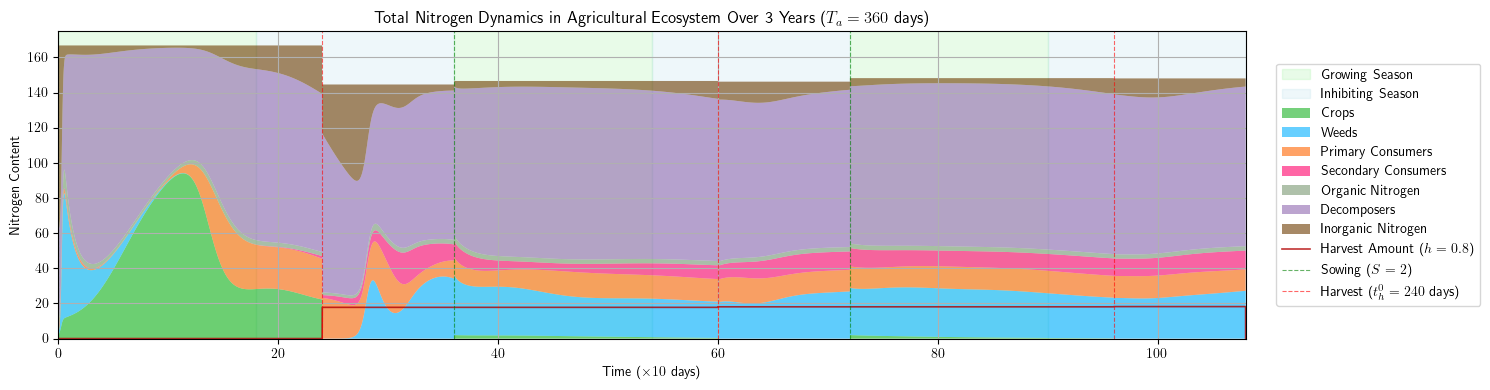
\includegraphics[width=\textwidth]{figures/model2_no_chem.png}
\setlength{\abovecaptionskip}{-0.5cm}
\caption{Agricultural ecosystem without chemicals}
\label{fig:model2_no_chem}
\end{figure}

Furthermore, we can also observe that after the first harvest, the inorganic nitrogen content in the environment remains relatively stable, and the total harvest of crops has been at an almost constant low level. This phenomenon is mainly due to two reasons: first, the rapid proliferation of primary consumers, namely pests, causes severe damage to the crops, leading to reduced yields; second, the fast reproduction rate of weeds gives them an advantageous position in interspecific competition, which inhibits the growth of crops. Therefore, to increase crop yields and enhance the stability of the agricultural ecosystem, it is necessary to use chemical substances to ensure the efficiency, safety, and stability of agricultural production, and we will discuss in detail the impact of herbicides and pesticides on the agricultural ecosystem in the following section.
\subsubsection{Herbicides and Insecticides}  

In the agricultural cycle, weeding and pest control are also essential steps. Herbicides and insecticides are commonly used chemicals that play an important role in increasing crop yields and reducing competition from pests and weeds. We assume that herbicides mainly affect the mortality rate of weeds, while insecticides primarily affect the mortality rate of pests, or primary consumers. Based on equation (\ref{eq:model2_season}), we establish the following equation:
\begin{align}
\begin{cases}    
    \displaystyle \vspace{10pt}
    \gamma _w\left( t \right) =\gamma _{w}^{0}+
    \boxed{\gamma _{w}^{\text{chem}} e^{-\lambda _w\left( t-T_wn_w \right)}\cdot I_{\{N_c > 0\}}}
    +\gamma _{w}^{s}\sin \left( \frac{2\pi t}{T}+\phi + \pi \right) 
    \\\displaystyle
    \gamma _1\left( t \right) =\gamma _{1}^{0}
    +\boxed{\gamma _{1}^{\text{chem}}e^{-\lambda _1\left( t-T_1n_1 \right)}\cdot I_{\{N_c > 0\}}} 
    + \gamma_1^{s}\sin \left( \frac{2\pi t}{T}+\phi \right)
    \end{cases}
    \label{eq:model2_chem_deathRate}
\end{align}
where
\begin{itemize}  
    \item $\gamma_w^{chem}$, $\gamma_1^{chem}$, $\lambda_w$, and $\lambda_1$ are adjusted according to the mortality rates caused by the use of herbicides or insecticides, and these factors also exhibit periodicity;  
    \item $T_w$ and $T_1$ represent the cycles for the use of herbicides and insecticides, respectively, while $n_w$ and $n_1$ denote the counts of these two cycles.  
    \item The function $I_{\{N_c > 0\}}$ is an indicator function, which takes the value of 1 when the condition $N_c > 0$ is satisfied and 0 otherwise. It represents the presence or absence of crops, with pest control and weed removal occurring only when crops are present.  
\end{itemize}  

\subsubsection{Fertilization - Artificial Nitrogen Sources}

As shown in Figure (\ref{fig:Agriculture_cycle}), the fertilization process is located in the third stage of the agricultural cycle, a human-dominated process that supplements nitrogen in the agricultural ecosystem. Here, we mainly explore the impact of nitrogen fertilizers. Therefore, based on equation (\ref{eq:model2_environment}-3), we establish the following equation:
\begin{align}  
\frac{\mathrm{d}N_{inorg}(t)}{\mathrm{d}t} =&  \left( d - \delta \right) N_D(t) N_{org}(t) - r_w N_{inorg}(t) N_w(t) - r_c N_{inorg}(t) N_c(t) \nonumber\\  
&+\boxed{F \cdot \delta_D\left(t-n_fT_f-t_{f}^{0} \right) \cdot I_{\{N_c > 0\}}}  
\label{eq:model2_fertilize}  
\end{align}  
where
\begin{itemize}  
    \item $F$ represents the amount of fertilizer applied in one instance, $T_f$ represents the duration of fertilization cycle, $n_f$ denotes the count of fertilization cycles, and $t_{f}^{0}$ indicates the starting time of fertilization.  
\end{itemize}  

We can also define the input function for artificial nitrogen sources, $I(t)$:  
\begin{align}  
    I(t) = \int_0^t F \cdot \delta_D\left(x-n_fT_f-t_{f}^{0} \right) \cdot I_{\{N_c > 0\}}  + S\delta _D\left( x-t_{s}^{0}-T_an_a \right)\mathrm{d}x  
    \label{eq:input_function}  
\end{align}  
This function represents the total amount of fertilization applied from time 0 to $t$, reflecting all the inorganic nitrogen input.  

\subsection{The Evolution from Forest Ecosystem to Agricultural Ecosystem}  
In the process of transitioning from a forest ecosystem to an agricultural ecosystem, we consider dividing the discussion into two parts: biological and abiotic components.  

For the biological component, which includes the food chain and decomposers of the ecosystem, we can observe from the nitrogen cycle model of the forest ecosystem that there is a close material and energy flow relationship between these three elements. Human activities such as deforestation directly reduce the species richness of producers, which indirectly causing a sharp decrease in consumer populations. Therefore, the resistance stability of agricultural ecosystem weakened but the resilience stability enhanced.  

For the abiotic component, we mainly consider the content of soil organic matter (SOM). Aspects such as sunlight and air are not discussed here. Studies have shown that without proper measures to protect SOM, converting forests into agricultural land leads to degradation of soil physical and rheological properties \cite{SOW}. We believe that in agricultural ecosystems, the content of inorganic nitrogen and other substances available to producers in the soil decreases.  

In summary, the evolution from forest to farmland is a process where all stages of the nitrogen cycle undergo changes.

\section{Model 3: Agricultural Ecosystem-Food Web-Nitrogen Cycle Model}
In the previous section, we developed an Agricultural Ecosystem Nitrogen Cycling Model (AENCM), integrating the competition between crops and weeds, as well as human-induced impacts. However, in the AENCM, we assumed that during the early stages of agricultural ecosystem establishment, higher trophic consumers that once inhabited the forest would migrate due to habitat loss and human activities. As a result, we considered a simplified two-tier consumer food chain.

Over time, as the agricultural ecosystem stabilizes, native species gradually return to the system \cite{LAFEVOR201432}. With the re-establishment of higher trophic consumers, the simplistic food chain model is no longer sufficient to describe the complex interrelationships within the agricultural ecosystem. Therefore, in this section, we extend the AENCM by incorporating the effects of a more intricate food web on the ecosystem.
\begin{figure}[ht] 
\centering
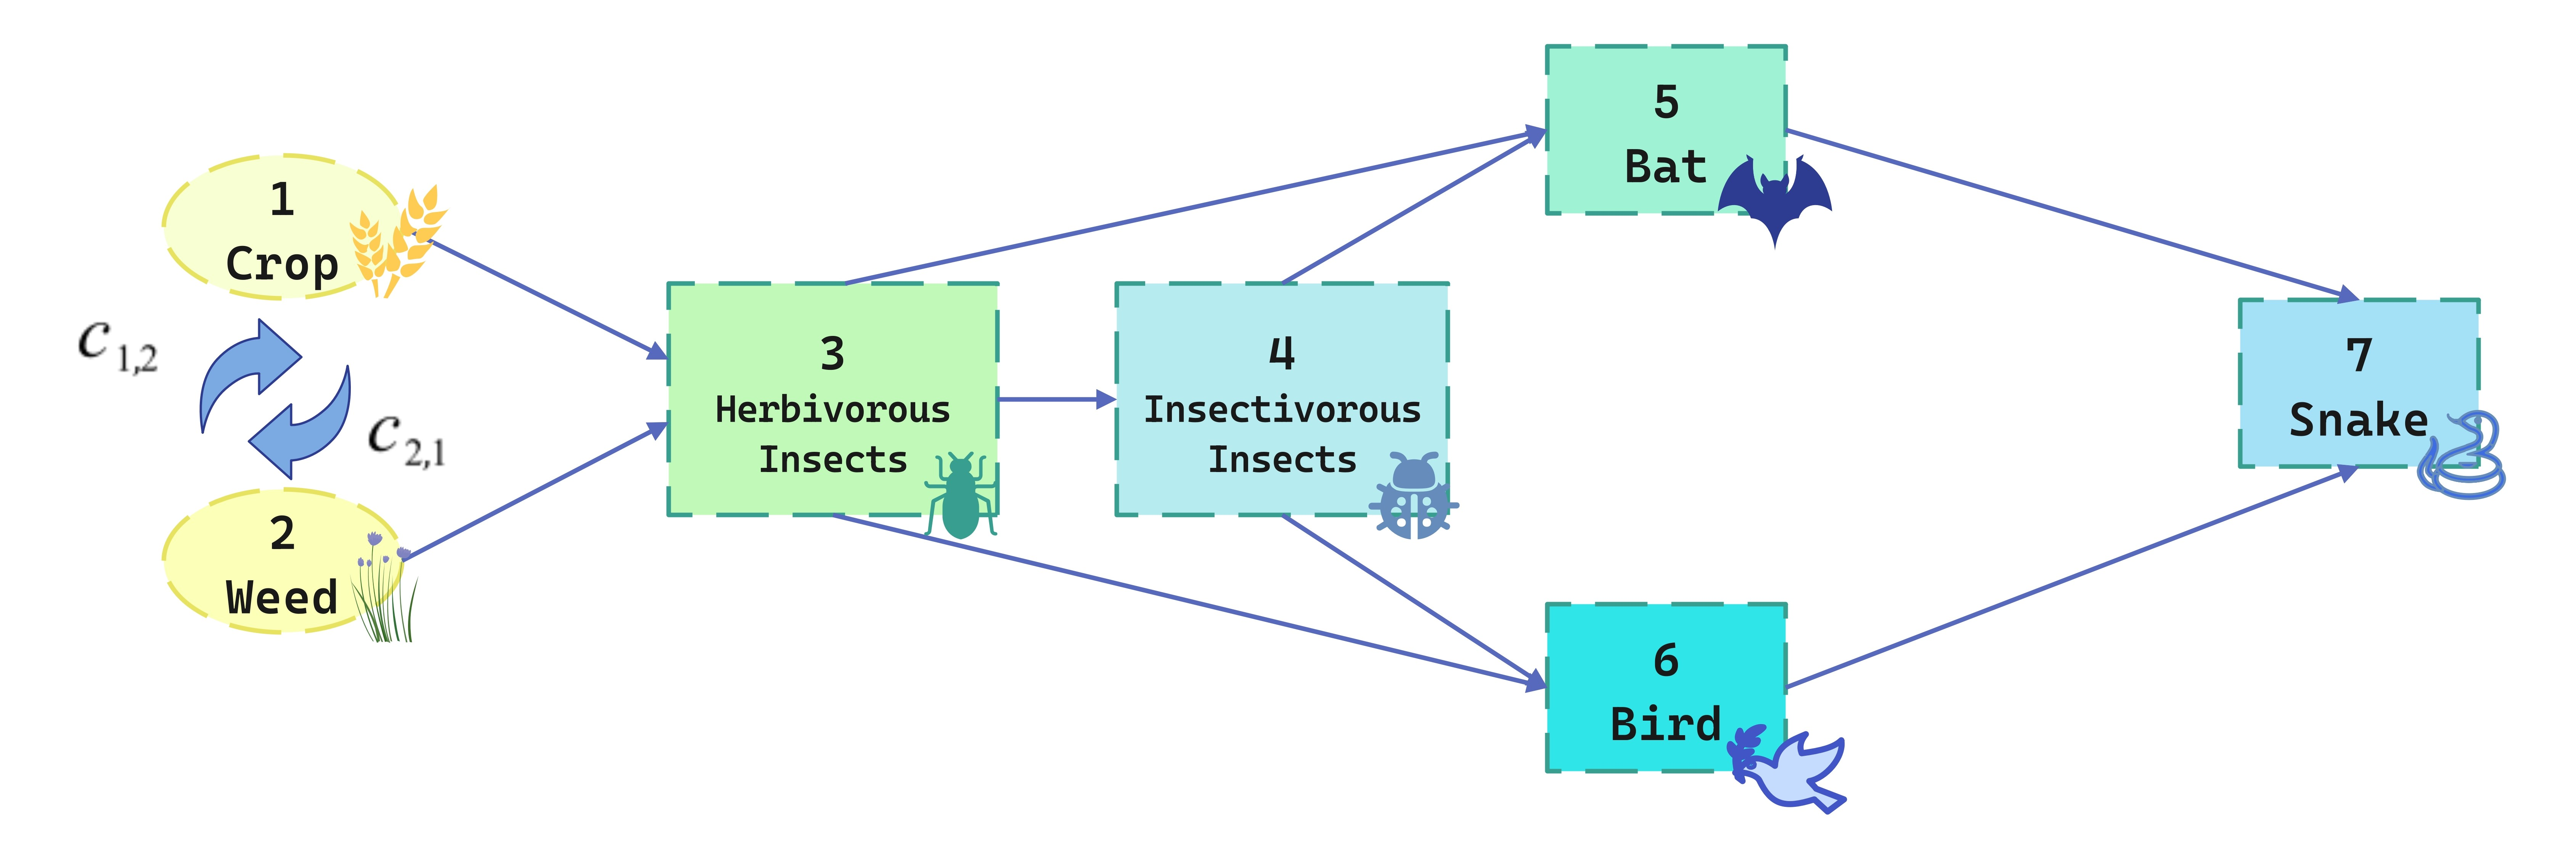
\includegraphics[width=14cm]{figures/food web.jpg}
\caption{Agricultural ecosystem food web}
\label{fig:Agricultural_ecosystem_food_web}
\end{figure}
\subsection{The Establishment of Food Web Model}
\subsubsection{Fundamental Concepts and Key Definitions in Food Web Model}\label{sec:6.1.1}
We have designed a complex food web structure consisting of seven species, as illustrated in Figure (\ref{fig:Agricultural_ecosystem_food_web}). For the predator-prey relationships within this food web, we can define the predator-prey interaction matrix $\mathbf{P}_{7\times 7}$, the predation rate matrix $\mathbf{A}_{7\times 7}$, and the conversion efficiency matrix $\mathbf{B}_{7\times 7}$.
\begin{align}
\mathbf{P}_{7\times 7} = 
\begin{bmatrix}
0 & 0 & 1 & 0 & 0 & 0 & 0 \\
0 & 0 & 1 & 0 & 0 & 0 & 0 \\
0 & 0 & 0 & 1 & 1 & 1 & 0 \\
0 & 0 & 0 & 0 & 1 & 1 & 0 \\
0 & 0 & 0 & 0 & 0 & 0 & 1 \\
0 & 0 & 0 & 0 & 0 & 0 & 1 \\
0 & 0 & 0 & 0 & 0 & 0 & 0 
\end{bmatrix}, \quad \,\,
\mathbf{A}_{7\times7} =
\begin{bmatrix}
0 & 0 & \alpha_{1,3} & 0 & 0 & 0 & 0 \\
0 & 0 & \alpha_{2,3}  & 0 & 0 & 0 & 0 \\
0 & 0 & 0 & \alpha_{3,4} & \alpha_{3,5} & \alpha_{3,6} & 0 \\
0 & 0 & 0 & 0 & \alpha_{4,5} & \alpha_{4,6} & 0 \\
0 & 0 & 0 & 0 & 0 & 0 & \alpha_{5,7} \\
0 & 0 & 0 & 0 & 0 & 0 & \alpha_{6,7} \\
0 & 0 & 0 & 0 & 0 & 0 & 0 
\end{bmatrix}.
\end{align}
Here the element $(p_{ij})$ in $\mathbf{P}_{7\times7}$ is equal to 1 if species $i$ is preyed upon by species $j$, and 0 otherwise, indicating the absence of a predator-prey relationship. The matrix $\mathbf{A}_{7\times7}$ stores the corresponding predation rates $(\alpha_{ij})$ at the same positions as those in $\mathbf{P}_{7\times7}$. Similarly, $\mathbf{B}_{7\times7}$, structured like $\mathbf{A}_{7\times7}$, holds the corresponding predation conversion rates $(\beta{ij})$, which is omitted here for brevity.

Simultaneously, we can define the natural mortality rate vector of species $\Gamma_{7\times1}(t)$: 
\begin{align*}
    \Gamma_{7\times1}(t)= (\gamma_1(t), \gamma_2(t), \gamma_3(t), \gamma_4(t), \gamma_5(t), \gamma_6(t) ,\gamma_7(t))^\intercal
\end{align*}
where the elements of $\Gamma_{7\times1}(t)$ are expressed as $\gamma_i(t) = \gamma_i^0 + \gamma_i^{chem}(t) - \gamma_i^s \sin\left(\frac{2\pi}{T} + \phi\right)$, representing the natural mortality rate of species $i$ at time $t$, influenced by seasonal periodic fluctuations and the impact of artificial chemicals, similar to equation (\ref{eq:model2_chem_deathRate}).

The nitrogen content vector of species $\mathbf{N}_{7\times1}(t)$ is expressed as follows:
\begin{align*}
    \mathbf{N}_{7\times1}(t) = (N_1(t) , N_2(t) , N_3(t) , N_4(t) , N_5(t) , N_6(t) , N_7(t) )^\intercal
\end{align*}
where the element $N_i(t)$ in $\mathbf{N}_{7\times1}(t)$ represents the nitrogen content within species $i$ of the ecosystem, and this metric can also be used to indicate population abundance.

Similarly, we can define a competition coefficient matrix to represent the interspecific competition relationships and their intensities $\mathbf{C}_{7\times7}$.
\begin{align*}
\mathbf{C}_{7\times7} = 
    \begin{bmatrix}
        \begin{matrix} 0 & c_{1,2} \\ c_{2,1} & 0 \end{matrix} & \mathbf{O}_{2\times5} \\
        \mathbf{O}_{5\times2} & \mathbf{O}_{5\times5}
    \end{bmatrix}
\end{align*}
where the element $(c_{ij})$ in the above matrix $\mathbf{C}$ represents the competitive mortality rate inflicted on species $j$ by species $i$. If $(c_{ij}) = 0$, it indicates that species $i$ does not exert competitive pressure on species $j$. In our model, for computational simplicity, we only consider the competition between crops and weeds. To account for more intricate competitive interactions within the food web, one can directly adjust the values within the matrix.

Finally, we must define the vector representing the utilization efficiency of inorganic nitrogen by producers within the food web $\mathbf{R}_{7\times1}(t)$.
\begin{align*}
    \mathbf{R}_{7\times1}(t) = (r_1(t), r_2(t), 0,0,0,0,0)^\intercal.
\end{align*}
In the equation above, if an element $(r_{ij})$ in the vector $\mathbf{R}_{7\times1}(t)$ is nonzero, it indicates that species $i$ is a producer. The term $r_i(t)$ represents the rate where species $i$, as a producer, absorbs inorganic nitrogen from the environment, and can be used as a measure of the population growth rate of the producer.

\subsubsection{Agricultural Ecosystem Food Web-Nitrogen Flux Model}
After defining the symbols for the variables and parameters required in the food web, we can express the nitrogen flux equations within the food web as a system of differential equations in the following matrix form:
\begin{align*}
    \frac{\mathrm{d}\mathbf{N}\left( \boldsymbol{t} \right)}{\mathrm{d}\boldsymbol{t}}
    =-(\boldsymbol{AN}\left( t \right) )^\intercal \boldsymbol{N}\left( t \right) + (\boldsymbol{B}^{\intercal}\boldsymbol{N}\left( t \right) )^\intercal \boldsymbol{N}\left( t \right) -(\boldsymbol{C}^{\intercal}\boldsymbol{N}\left( t \right) )^\intercal \boldsymbol{N}\left( t \right) +
\boldsymbol{R}^\intercal \boldsymbol{N}\left( t \right) N_{inorg}-\Gamma \left( t \right)^\intercal \boldsymbol{N}\left( t \right)
\end{align*}

In the above equation, “$\mathbf{M}^\intercal$” denotes the transpose operation applied to the matrix $\mathbf{M}$. Simplifying further, we obtain the complete system of equations for the nitrogen flow model in the food web:
\begin{align}
    \frac{\mathrm{d}\mathbf{N}\left( \boldsymbol{t} \right)}{\mathrm{d}\boldsymbol{t}}
    =\big[ -\boldsymbol{AN}\left( t \right) +\boldsymbol{B}^{\intercal}\boldsymbol{N}\left( t \right) -\boldsymbol{C}^{\intercal}\boldsymbol{N}\left( t \right) +N_{inorg}(t)\boldsymbol{R}- \Gamma \left( t \right) \big]^\intercal  \boldsymbol{N}\left( t \right) 
    \label{eq:model3_food_web}
\end{align}

In the equation above, $\mathbf{N}(t)$ represents an $n$-dimensional column vector. The equation depicts the dynamics of nitrogen flux among $n$ species within the food web. Here, $N_{inorg}(t)$ denotes the concentration of inorganic nitrogen in the environment at time $t$. Through this variable, we can establish connections between the aforementioned equation and the organic nitrogen, inorganic nitrogen, and decomposer equations in Model 2. Additionally, it allows for the incorporation of anthropogenic factors such as sowing, harvesting, weeding, pest control, and fertilization, ultimately resulting in the comprehensive Agricultural Ecosystem-Food Web-Nitrogen Cycle Model (AE-FW-NCM).

\subsubsection{Evaluating Agricultural Ecosystems}
Before we start to solve the AE-FW-NCM, we need to define two indicators to evaluate agricultural ecosystems comprehensively. These indicators will help us understand the stability and efficiency of nitrogen cycling within the ecosystem.

Firstly, we define the average nitrogen transformation efficiency over a period of time as an indicator of ecosystem stability. The definition of this indicator is as follows:
\begin{align}
\mu_N = \int_{t_0}^{t_0+\Delta t} \frac{(r_1(x)N_1(x) + r_2(x)N_2(x))N_{inorg}(x)}{\sum N_i(x) + N_{inorg}(x) + N_{org}(x) + N_D(x)}  \mathrm{d}x
\label{eq:evaluate_ecosystem}
\end{align}
where 
\begin{itemize}
    \item the numerator represents the rate at which producers convert inorganic nitrogen to organic nitrogen at a given moment,
    \item the denominator represents the total amount of nitrogen in the ecosystem at that moment,
    \item By integrating over a certain time period, the nitrogen transformation efficiency for that period can be obtained.
\end{itemize}
Secondly, by combining equations (\ref{eq:harvest_function}, 
\ref{eq:input_function}), the average nitrogen input-output conversion rate $\eta(t)$ can be defined.
\begin{align}
    \eta_{IO}(t) = \frac{H(t)}{I(t)}
    \label{eq:IO_rate}
\end{align}
which can be used to measure the economic utility of the agricultural ecosystem.

\subsubsection{Numerical Solution of the AE-FW-NCM}
By solving the system of equations (\ref{eq:model2_environment}, \ref{eq:organic_nitrogen_with harvest}, \ref{eq:model2_fertilize}, \ref{eq:model3_food_web}) simultaneously, we are able to simulate the complete nitrogen cycle within agricultural ecosystem. Employing the Euler Method for the discrete solution of the system of differential equations, we can generate visual representations, as illustrated in Figure(\ref{fig:model3_foodWeb_2Chem}).
\begin{figure}[ht] 
\centering
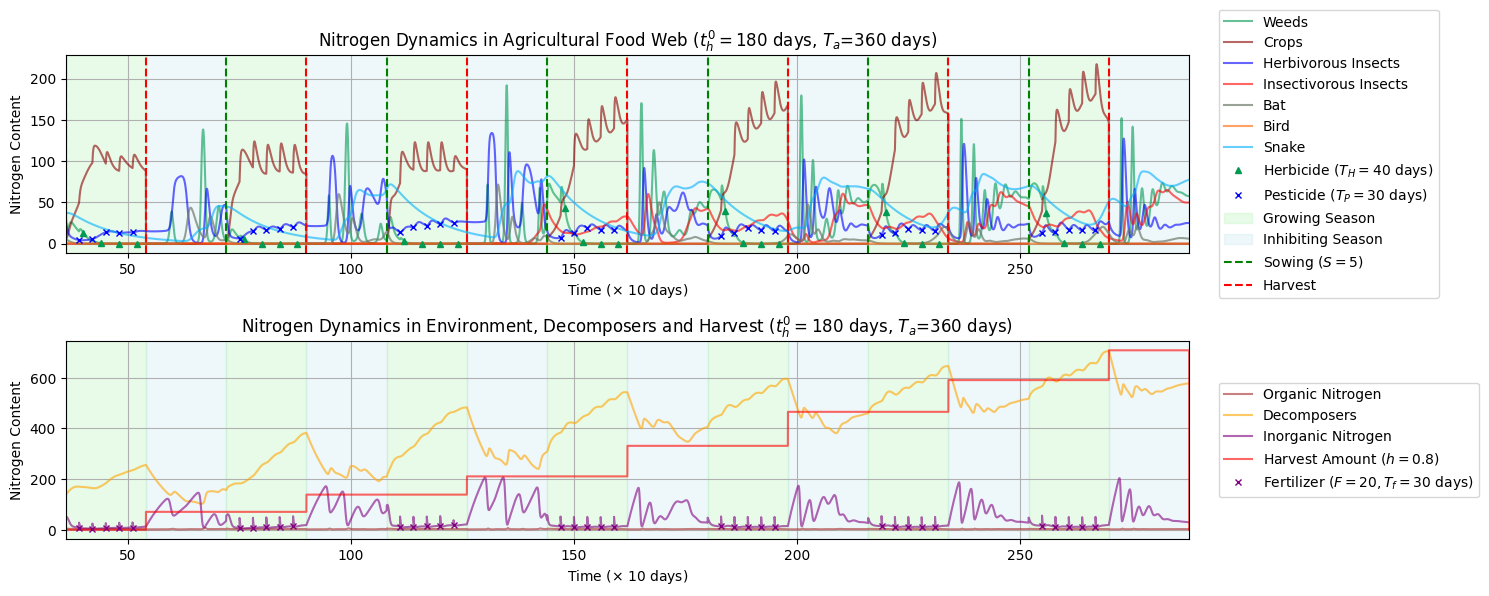
\includegraphics[width=\textwidth]{figures/model3_food_web_2Chem.png}
\setlength{\abovecaptionskip}{-0.5cm} 
\caption{Agricultural Ecosystem-Food Web-Nitrogen Cycle}
\label{fig:model3_foodWeb_2Chem}
\end{figure}

In the figure above, due to the instability of the first-year simulation results, the nitrogen cycle during the agricultural cultivation process is depicted starting from the second year ($\text{Time}_0 = 36 \, \times 10 \text{days}$), spanning a total of 7 years. It can be observed that, under the application of herbicides and insecticides, crops quickly gain dominance during the planting period in each cycle, resulting in a consistently high crop yield each year. 

The calculations show that when both herbicides and insecticides are used, the nitrogen input-output conversion rate (\(\eta_{\text{IO}}\)) over seven years is 80.945\% (excluding the 20\% nitrogen content remaining in the straw after harvest). However, the nitrogen transformation efficiency (\(\mu_N\)) is only 13.12\%, indicating poor ecosystem stability.

Although chemicals boost crop yields, they also bring significant economic and labor costs and pose environmental risks. The next section will explore the impacts of chemical use and potential alternatives.
\subsection{The Impact of Chemicals}
\subsubsection{The Impact of Chemicals on the Stability of Ecosystems}
The impact of chemicals on the stability of agricultural ecosystems is a complex issue.Specifically, as discussed in the previous section, herbicides and pesticides, although commonly regarded in agriculture as effective tools for increasing crop yields and controlling pests, can result in long-term negative effects on ecosystems. 

(1) Impact on Soil: Excessive use of fertilizers may lead to soil acidification, salinization, and nutrient imbalances. Beneficial microbial communities may be inhibited by these chemicals, affecting soil fertility and its natural restorative capacity. 

(2) Impact on Producers: As illustrated in the Figure(\ref{fig:model3_foodWeb_2Chem}), the introduction of herbicides and insecticides promotes crop growth, with total harvest levels remaining consistently high and stable. Furthermore, both weed and pest populations significantly decline. 

(3) Impact on Consumers at Various Trophic Levels: The use of herbicides and insecticides in agricultural practices directly affects primary consumers. Moreover, studies suggest that agricultural chemicals ultimately influence higher trophic levels through bioaccumulation. Specifically, chemical molecules tend to adsorb onto microplastic particles, enhancing their toxicity and destructive impact on biological cells.\cite{bioaccumulation}.

(4) Impact on Ecosystems: The widespread use of chemicals may adversely affect species diversity and ecological balance within agricultural ecosystems. 
\begin{figure}[ht] 
\centering
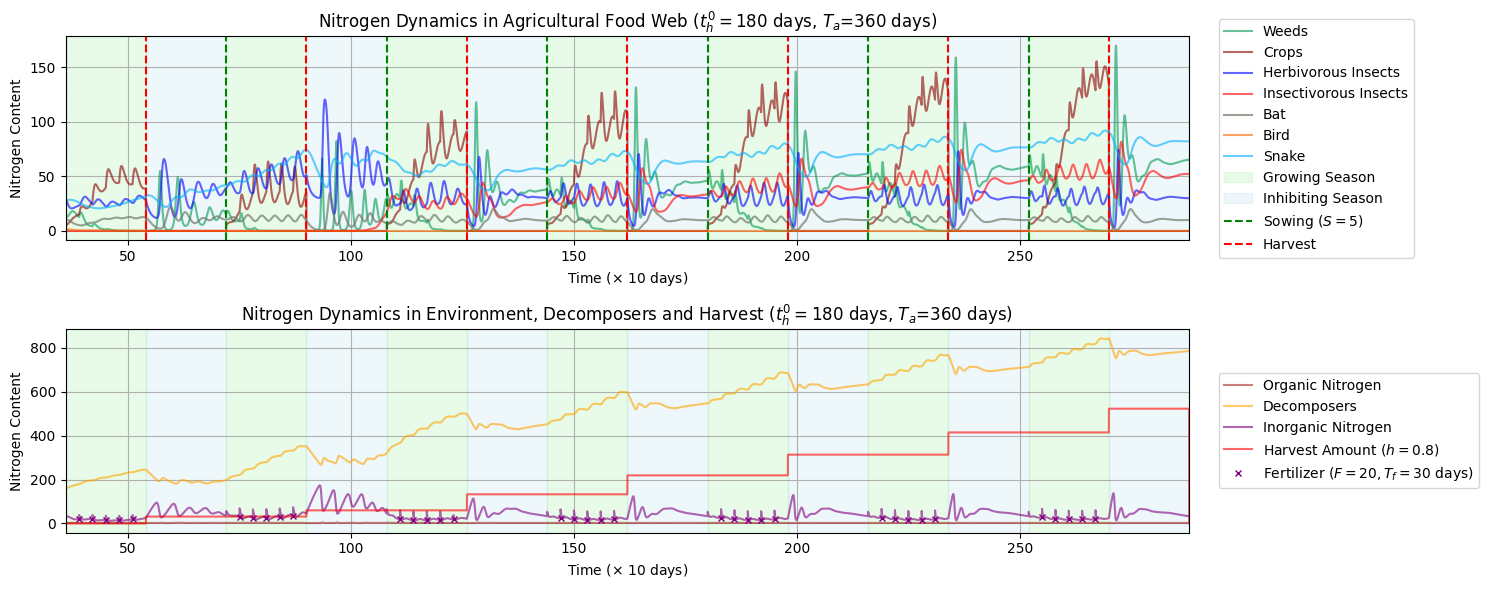
\includegraphics[width=\textwidth]{figures/model3_food_web_noChem.png}
\setlength{\abovecaptionskip}{-0.5cm} 
\caption{AE-FW-NCM without Chemicals}
\label{fig:model3_foodWeb_noChem}
\end{figure}

\subsubsection{Clearance of Herbicides and Insecticides}
Given the potential environmental hazards posed by the use of chemicals such as herbicides and pesticides, as well as the substantial human and economic costs associated with their application, we considered the possibility of eliminating chemical usage.

By employing the same parameters as those used in the model depicted in Figure(\ref{fig:model3_foodWeb_2Chem}), but excluding herbicides and pesticides, we obtained the simulation results shown in  Figure(\ref{fig:model3_foodWeb_noChem}). The data reveal that, even after disregarding the highly unstable first year, nitrogen levels across various populations demonstrate a consistent upward trend over time. Crop yields similarly increase year by year, eventually stabilizing.

Furthermore, using equation(\ref{eq:IO_rate}), we calculated the nitrogen input-output ratio to be 59.68\%. In comparison to the results with chemical use, it is likely that the absence of chemicals allows for a higher carrying capacity of species within the food web, thereby requiring a greater nitrogen input to achieve population equilibrium. And using Equation (\ref{eq:evaluate_ecosystem}), we can calculate that \(\mu_N = 14.29\%\), which indicates that the ecosystem is more stable when no chemicals are used.
\subsection{Biological Control}
\subsubsection{Consideration of Bat Pollination}
As the second-largest group of mammals globally, approximately 70\% of bat species serve as essential insect predators, consuming up to 80-100\% of insects each night. This contributes significantly to pest control in agriculture. Bats typically venture out at night, and due to their unique navigation abilities, they often carry plant pollen and seeds, thereby aiding in the reproduction of crops within agricultural ecosystems\cite{bat_seed}.

In the previous simulation, we only considered the role of bats in pest control. In this section, we expand the model to also account for bats' contribution to crop reproduction. Building upon the notation in \ref{sec:6.1.1}, and based on equation(\ref{eq:model2_season}), we can establish the following equation:
\begin{align}
    r_1(t)  = r_{1}^{0} + r_{1}^{s}\sin \left( \frac{2\pi t}{T}+\phi \right) + r_1^{bat}N_5(t)
\end{align}
where $r_1$ denotes the rate at which crops utilize nitrogen, $r_1^{bat}$ denotes the facilitation coefficient of bats on crop growth, $N_5(t)$ indicates the total nitrogen content in the bat population, which can be approximated as an indicator of bat population size.
\begin{figure}[ht] 
\centering
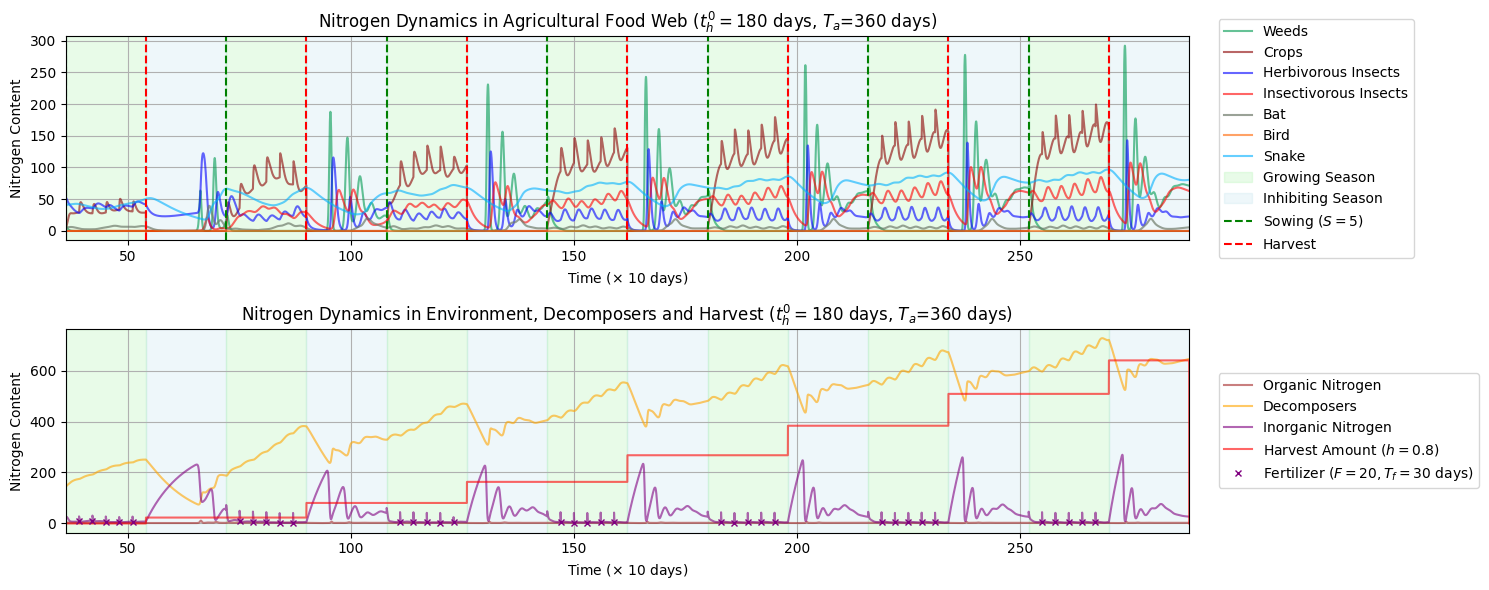
\includegraphics[width=\textwidth]{figures/model3_food_web_Bat.png}
\setlength{\abovecaptionskip}{-0.5cm} 
\caption{Bats Promote Crop Reproduction ($r_1^{bat} = 0.05$)}
\label{fig:model3_foodWeb_bat}
\end{figure}

After considering the role of bats in promoting crop reproduction, we set the parameter $r_1^{bat} = 0.05$, as depicted in Figure(\ref{fig:model3_foodWeb_bat}). Then we calculated the $\eta_{IO}$ and $\mu_N$, which were found to be 72.89\% and 14.62\%. It can be observed that both the economic benefits and the stability of the ecosystem are superior when bats are considered in the model.

\subsubsection{Another Species for Biological Control}
Given the crucial role bats play in agricultural ecosystems, we identified another species with a similar ecological function— Chrysoperla—through a thorough review of relevant literature.  Chrysoperla, widely recognized as natural beneficial insects, are renowned for their ability to prevent aphid infestations\cite{Turquet2009BiologicalCO}.

(1) Similarities: Both bats and Chrysoperla larvae reduce pest populations in crops by preying on harmful insects, thereby enhancing crop yields. Bats primarily target flying insects, while Chrysoperla mainly feed on common agricultural pests such as aphids. 

(2) Differences: First, bats primarily prey on flying pests, whereas Chrysoperla target ground-dwelling or plant-based pests. Additionally, bats contribute to pollination and seed dispersal while Chrysoperla are generally regarded solely as pest controllers. Finally, bats require specific habitat conditions. However, Chrysoperla exhibit greater environmental adaptability and are easier to manage, with populations typically remaining stable.

\section{Green Agriculture}
Green agriculture refers to an agricultural model that leverages scientific advancements or natural principles to achieve sustainable development within agricultural production. Based on the agricultural cycle processes and key nitrogen cycle stages outlined in the aforementioned research, we provide a detailed analysis of green agriculture development from the following perspectives.

\subsection{Nitrogen fixation — Rhizobium and Soybeans}
Certain specialized microorganisms, known as nitrogen-fixing bacteria, possess the unique ability to convert nitrogen gas into inorganic salts that plants can utilize. Therefore, their application in agriculture could provide a natural and continuous supply of nitrogen fertilizer.

In practical agricultural applications, rhizobia and soybeans, as typical symbiotic organisms in nature, contribute their nitrogen fixation abilities to the soybean cultivation process. Research has confirmed that treatment with rhizobia significantly enhances both the number of pods per plant and the annual yield. In nature, however, the nitrogen-fixing capacity of these bacteria benefits more than just leguminous crops. Gramineous plants can also engage in symbiosis with rhizobia. For instance, a novel species of Rhizobium, R. oryzae, isolated from wild rice (Oryza alta), demonstrates that certain rhizobia serve as endophytes in grasses and can promote rice yield. Additionally, non-leguminous plants often form nitrogen-fixing symbiotic relationships with Frankia actinobacteria.\cite{genliujun}

\subsection{Recycling and Utilization – Straw} 
\label{sec:crops_residue}
In our model(Eq.\ref{eq:harvest_function}), it has been observed that a portion of organic nitrogen within the crops is removed from the ecosystem along with the harvest, yet remains underutilized. The quantity of this unexploited organic nitrogen can be calculated as follows:
\begin{align}
    N_{straw}(t) = \frac{(1-h)H(t)}{h}
\end{align}

In agricultural practices, a substantial amount of straw, particularly stems and stalks, remains after harvest.In reality, we believe a shift in perspective is needed. Rather than viewing straw as waste to be disposed of, it should be regarded as a valuable resource or raw material. We have compiled several viable strategies for the recycling of straws.

(1) As a substrate for mushroom production, the protein content of rapeseed straw fruiting bodies exceeds that of other substrates, making rapeseed straw highly suitable for oyster mushroom cultivation\cite{mushroom}.

(2) Integrated microbial degradation and enzymatic hydrolysis for the production of combustible gases. Straw has been widely used in biogas production. Simultaneous microbial degradation and enzymatic hydrolysis significantly enhance the efficiency of biogas conversion.\cite{CH4}

(3) Mechanized Composting. Straw composting involves adding animal manure and enzymes to the straw, followed by mixing with a lathe to homogenize the mixture\cite{gummert2020sustainable}. Compost can be used as a fertilizer for growing vegetables and other crops, enhancing soil nutrients and organic matter content.

\section{Sensitivity Analysis}
In Section \ref{sec:5_1}, we introduced the competition coefficients $c_{c,w}$ and $c_{w,c}$ between crops and weeds. In this section, by conducting sensitivity analysis on these two competition coefficients, it can be concluded that the growth of crops and nitrogen yield are insensitive to the competition coefficients when herbicides are applied. However, in the absence of herbicides, the growth of crops is more sensitive to the competition coefficients.
\begin{figure}[h]
    \centering
    \begin{subfigure}[b]{0.3\textwidth}
        \centering
        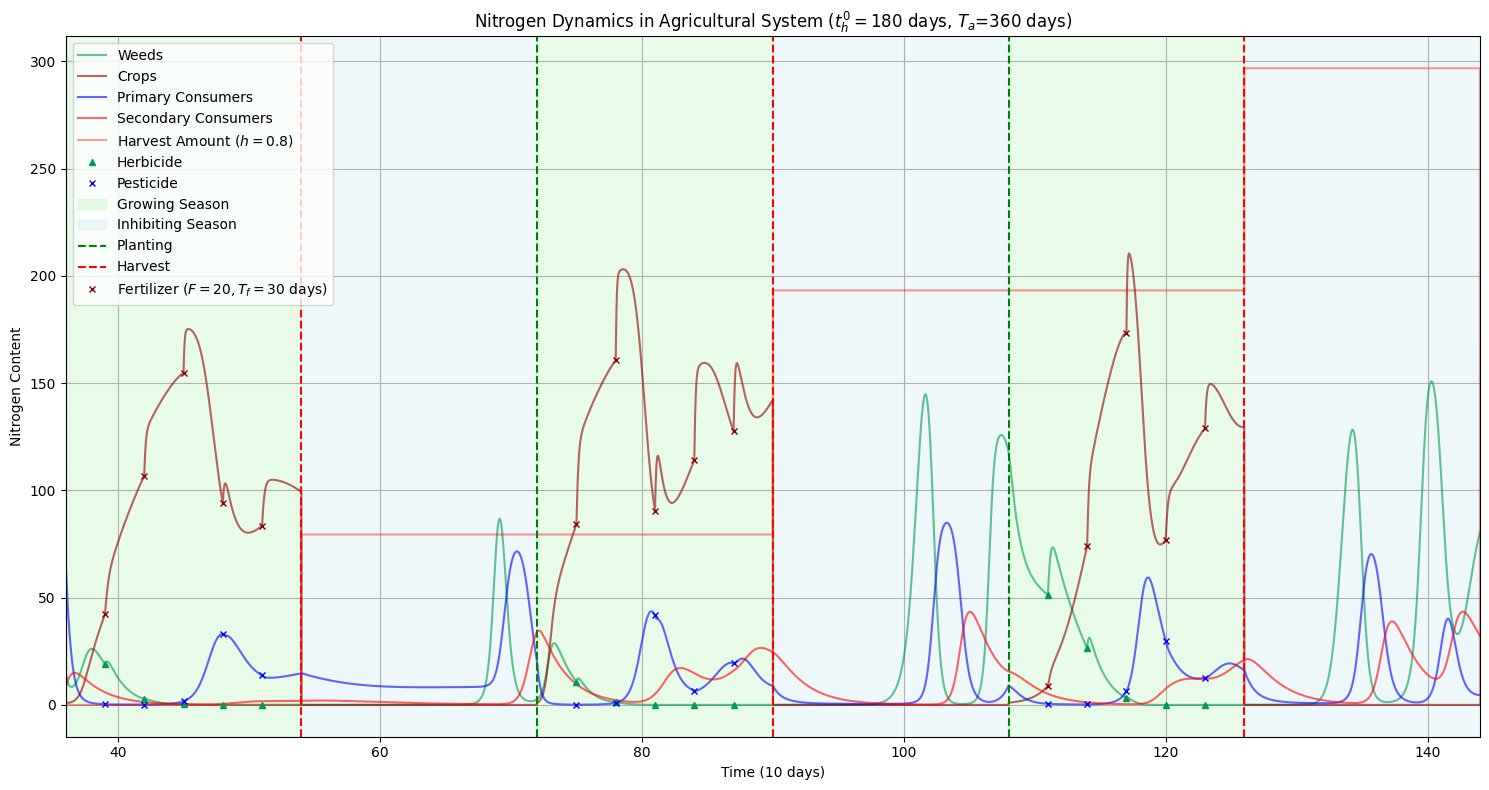
\includegraphics[width=\textwidth]{figures/fig_sensi_chem_2.png}
        \caption{Both}
        \label{fig:sensi_sub1}
    \end{subfigure}
    \hfill 
    \begin{subfigure}[b]{0.3\textwidth}
        \centering
        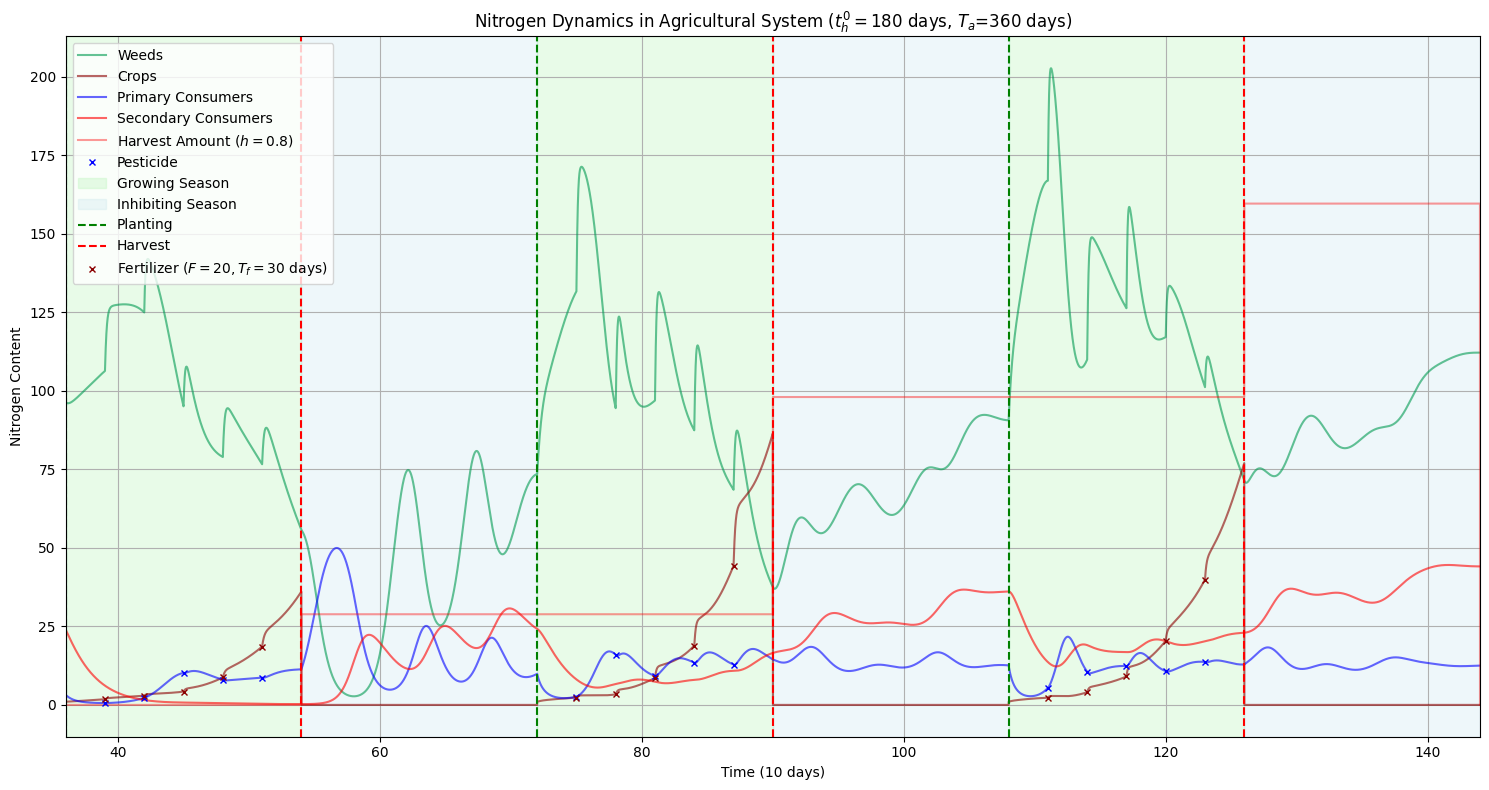
\includegraphics[width=\textwidth]{figures/fig_sensi_chem_1.png}
        \caption{Only Insecticides}
        \label{fig:sensi_sub2}
    \end{subfigure}
    \hfill 
    \begin{subfigure}[b]{0.3\textwidth}
        \centering
        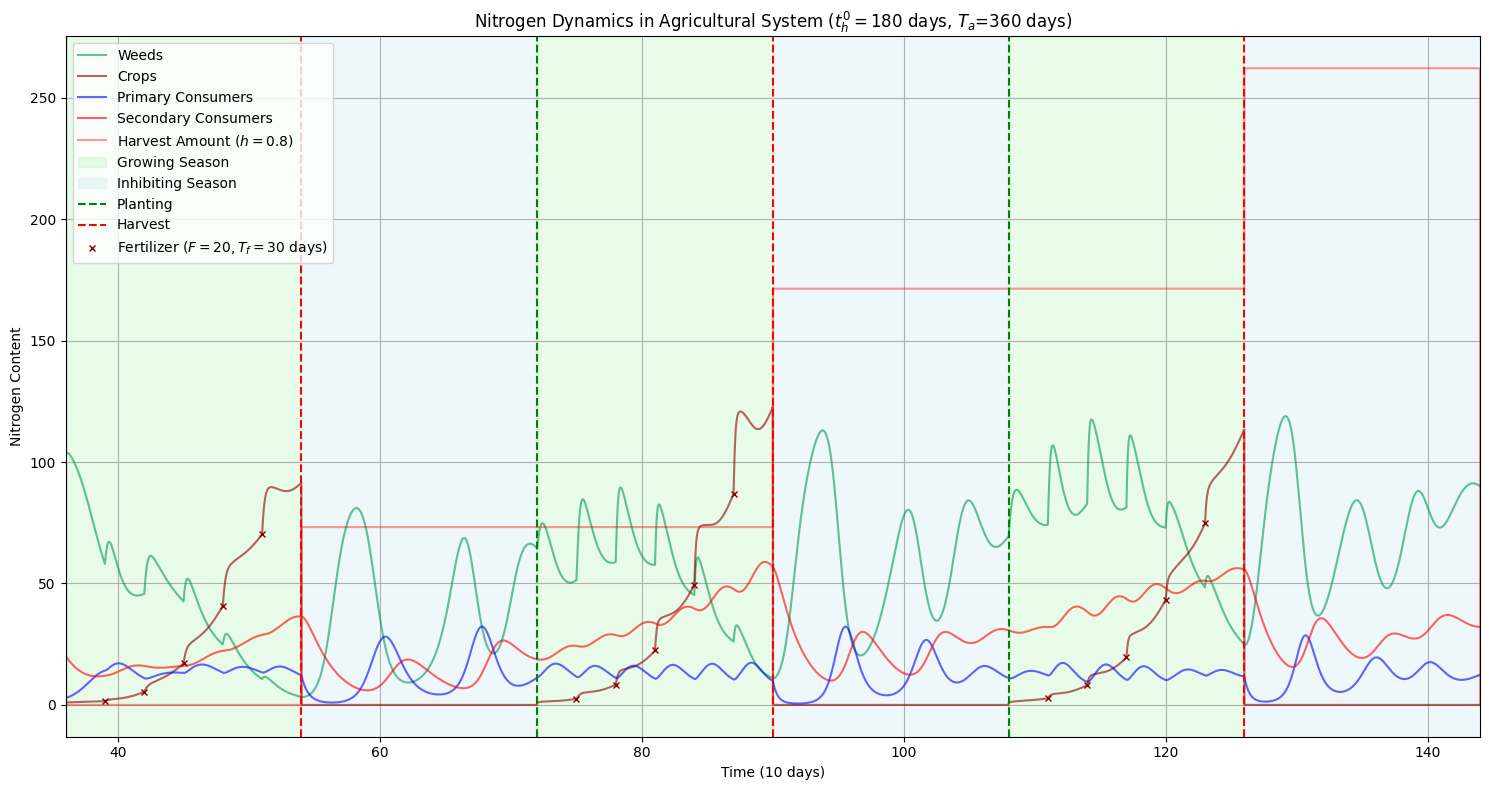
\includegraphics[width=\textwidth]{figures/fig_sensi_chem_0.png}
        \caption{Neither}
        \label{fig:sensi_sub3}
    \end{subfigure}
    \caption{The Impact of Chemical Use on Dominant Species}
    \label{fig:main}
\end{figure}

The competition coefficients in Figures (\ref{fig:sensi_sub1}, \ref{fig:sensi_sub2}, \ref{fig:sensi_sub3}) are $r_{c,w} = 0.002, r_{w,c} = 0.005$, comparing the changes in nitrogen content of various populations in the ecosystem under different chemical usage scenarios.

Furthermore, as shown in Figure (\ref{fig:sensi_competition}), it is evident that when both herbicides and insecticides are used, the sensitivity of the yield $H(t)$ to the competition coefficients is the lowest; whereas when only insecticides are used, the sensitivity of $H(t)$ to the competition coefficients is the highest.

\begin{figure}[h]
    \centering
    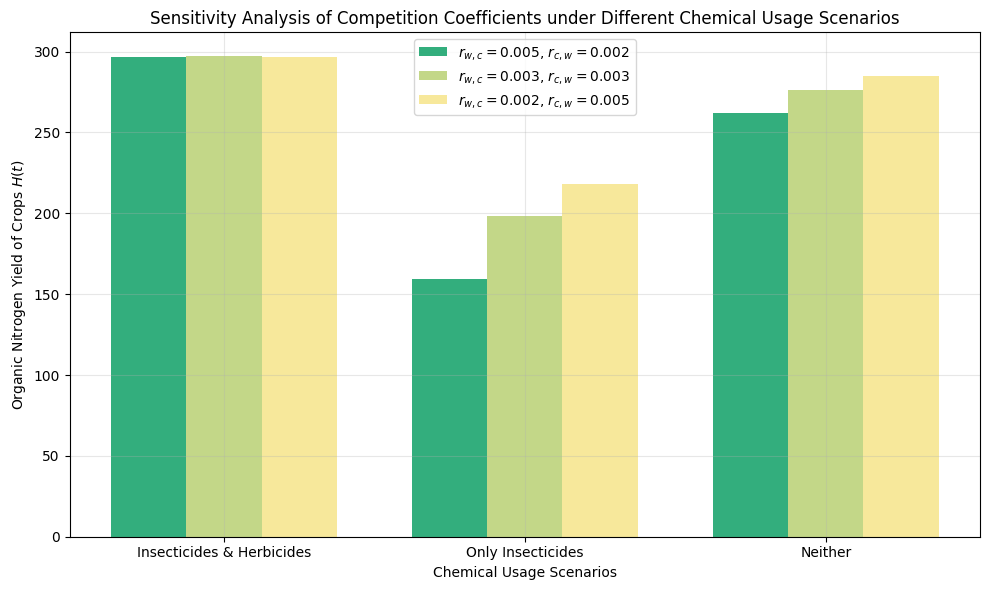
\includegraphics[width=0.5\linewidth]{figures/fig_sensitive.png}
    \caption{Sensitivity Between Harvest Amount and Competition Coefficients}
    \label{fig:sensi_competition}
\end{figure}

\section{Model Evaluation}
\subsection{Strengths}
\begin{itemize}  
    \item \textbf{Innovation.} We use nitrogen as a medium, treating the ecosystem as a whole for study. By analyzing the various stages of the nitrogen cycle within the ecosystem, we explore the different components of the ecosystem.  
    \item \textbf{Universality}. Our model endeavors to encompass a wide array of complex scenarios, such as the comprehensive simulation of the entire agricultural cycle in the AENCM, as well as the capability of Eq.\ref{eq:model3_food_web} to simulate any intricate food web.
    \item \textbf{Logic.} We start by creating an initial model for the forest ecosystem, then establish a model for the agricultural ecosystem based on the forest-to-farm transition, and finally add a food web model. The process progresses step by step, with strong logical coherence.  
    \item \textbf{Rigor.} Each step of our model update process is supported by theoretical foundations and is also corroborated by authoritative literature. 
\end{itemize}  
\subsection{Weakness and Further Discussion}
\begin{itemize}  
    \item In the available online literature and resources, we found insufficient data regarding the food web model of agricultural ecosystems. As a result, it is challenging to obtain accurate and stable parameter values, and parameter estimation may not be entirely precise.  
    \item In the future, we will focus on collecting more extensive and accurate data, continuously improving our model, and enhancing its adaptability in practical applications, thereby providing more reliable assistance for farmers practicing organic farming.  
\end{itemize}  


\printbibliography

\newpage

\begin{letter}{Dear Farmers,}  
%%%%%%%% Here begins the letter

We are writing to share some valuable research conclusions related to green agriculture. We are more than delighted to see that you are exploring organic farming practices and contributing to the sustainable development of agriculture on Earth! Our team has developed a nitrogen cycle model for agricultural ecosystems and conducted relevant research. Below, we offer some suggestions that we hope will aid your exploration:

\begin{itemize}  
\item Focus on the concept of agricultural ecosystems. Farmland is an integrated system comprising both biotic and abiotic environments, where a complete nitrogen cycle exists between the food chain and the inorganic environment. Therefore, maintaining the overall material cycling process is crucial for the stability of agricultural ecosystems. 
\item Control the usage of agricultural chemicals. Our research has shown that chemicals like herbicides and insecticides indeed have significant immediate effects on crop yields, but their excessive long-term use can greatly impact the stability of the agricultural ecosystem. For example, they can cause irreversible damage to the soil and, due to bioaccumulation, pose risks to human health.  
\item Use biological control methods wisely. Our model results indicate that the effectiveness of biological control in agricultural ecosystems is comparable to that of chemical agents, with the added advantage of sustainability. For instance, targeting pests using the behavioral characteristics of animals such as bats and ladybugs not only has long-term positive effects but also saves significant economic costs and increases yields.  
\item Recycle agricultural by-products. The large amount of straw left after crop harvest has immense potential for utilization. For example, straw remaining after wheat harvest can be used in various ways, such as in mushroom cultivation substrates, mechanized composting and returning to the soil, or microbial degradation and enzyme hydrolysis to produce combustible gases, all of which can bring significant economic benefits. 
\end{itemize}  

Sustainable organic farming practices are a long-term exploration process, and they rely on continuous research and practice by everyone involved. We sincerely hope that you can find the appropriate farming methods that suit your needs!

\vspace{\parskip}

Sincerely yours,  
Team \# 2515324.

\end{letter}


\newpage
\newcounter{lastpage}
\setcounter{lastpage}{\value{page}}
\thispagestyle{empty} 


% 重置页码
\clearpage
\setcounter{page}{\value{lastpage}}

\end{document}
